\chapter{心脏和大血管}

\section{检查方法}

\subsection{常规检查}

非心电门控常规CT扫描能用来显示心脏、心包和大血管的解剖形态。目前,心电门控常规CT扫描很少用来评价心脏功能。

1.平扫:一般采用层厚和间隔10mm,扫描范围大者如观察胸、腹主动脉瘤,可采用间隔15~20mm。

2.增强扫描:60%的复方泛影葡胺或非离子型造影剂80~100ml,团注、滴注或团注加滴注法。扫描方式分为常规扫描和动态扫描,后者又分为同层动态扫描和进床式动态扫描。

3.螺旋CT扫描:可采用平扫和增强扫描,并可进行三维重建。是否采用增强扫描,采用何种增强方式,视所检查部位和病变而定。如心包病变观察积液或钙化平扫即可,但不能确定是少量积液还是增厚时可增强扫描;主动脉病变特别是主动脉夹层时,应采用增强扫描;心腔内肿瘤或血栓平扫后作动态增强扫描以及延迟扫描,观察有无强化及其强化特点,以资鉴别。

\subsection{多层螺旋CT(MSCT)心功能检查}

多层螺旋CT扫描时间达亚秒级,接近电子束CT,其空间分辨率更高。可用于心脏功能部分参数的测定。

1.扫描时可采用以下参数:①扫描前测心率,并口服药物贝他洛克使心率降至70次/分钟以下;②注入60%造影剂120~160ml,流率3~3.5ml/s;③延迟时间25秒,层厚1.3mm左右,重建间隔0.6mm,螺距0.375~0.5;④扫描完成后对原始数据进行离线重建,取得8个R-R间期不同时相的图像(12.5%、25.0%、37.5%、50.0%、62.5%、75.0%、87.5%、100%);三维重建方式为SSD、MPR、VR。

2.心功能的测量方法:①冠状动脉测量:在单层横断面图像上分别找到显示左、右冠状动脉主支最佳处,在距开口1.0cm处分别测量左、右冠状动脉主支内径。②室间隔、室壁增厚率测量:将所得8个序列图像进行MPR处理,得到心室短轴位像。于左心室舒张末期和收缩末期分别测量左室前壁和室间隔的心肌厚度,并计算心肌增厚率(%)。计算公式为:心肌增厚率(%)=(EST-EDT)/EDT(EST为收缩末期厚度,EDT为舒张末期厚度),正常值>35%。室间隔与左室后壁舒张期厚度<11~12mm。③左室容积和射血分数测量法:以SSD方法分别对左心室舒张末期和收缩末期左室充盈区逐层勾画,最后由计算机自动计算左室舒张末期容积(EDV)和收缩末期容积(ESV)。左室射血分数(EF)计算公式为:EF(%)=(EDV-ESV)/EDV。EF正常值(67±8)%,范围50%~75%。

\subsection{大血管CTA}

1.颈动脉:扫描层厚2~3mm,造影剂用量90~150ml不等,流率2.5~3ml/s,扫描延迟时间15~20秒。三维重建方式:SSD、MIP和CPR。

2.胸主动脉:可采用心电门控扫描。层厚3~5mm,造影剂用量同上,流率2.5~3ml/s,扫描延迟时间15~20秒。三维重建方式:SSD、MIP和CPR。

3.腹主动脉:扫描层厚3~5mm(肾动脉可采用1.5~3mm),造影剂用量同上,流率2.5~3ml/s,扫描延迟时间20~25秒。三维重建方式:SSD、MIP和CPR。

4.肺动脉:扫描层厚3mm,重建层厚1.5mm,造影剂用量同上,流率3~3.5ml/s,扫描延迟时间10~16秒。扫描范围从主动脉弓至下肺静脉水平。三维重建方式:SSD和CPR,MIP影像重叠一般不采用。

5.冠状动脉:心电门控扫描。层厚1.25~1.5mm,重建间隔0.6mm,造影剂用量同上,流率3~4ml/s。扫描延迟时间15~20秒,可固定用18秒或小剂量(15~20ml)以3~4ml/s的流率预实验决定最佳延迟时间。三维重建方式:MPR、MIP、SSD、VR、VE,首选MIP。

国外有学者采用下列方法行MSCT冠脉检查:检查前舌下含化400μg硝酸甘油;先用20ml对比剂测定循环时间,根据循环时间确定开始扫描时间;然后以4ml/s的流率注入150ml(400mg/ml)对比剂。回顾性心电门控多层螺旋重建,右冠脉为R-R间期的38%~50%,左冠脉为R-R间期的50%。

\subsection{螺旋CT上腔静脉造影}

扫描层厚3~5mm,重建层厚1.5~2mm,造影剂用量80~100ml,流率2ml/s,扫描延迟时间25~30秒。扫描范围包括T\textsubscript{1}
椎体至右心房层面。三维重建方式:MPR、MIP和SSD。

\subsection{电子束CT的应用价值}

电子束CT(EBCT)有3种不同的扫描方式:①电影成像:用来测定左室总体和区域性功能;②流动成像:用作流量分析;③体积扫描:能测定心脏结构异常。

EBCT具有优良的时间分辨率,运动伪影大大减少。对于冠状动脉钙化显示的敏感性极高,还可作定量分析,能显示冠状动脉旁路是否通畅。同时可以通过旋转和倾斜检查床,使病人心脏的长轴或短轴与X线束垂直或平行,以得到真正的心脏短轴或长轴图像。但其价格昂贵、维修复杂,目前尚未被广泛应用。

\section{正常解剖和CT表现}

\subsection{心脏各房室的形态}

心脏由4个房室腔组成。①右心房:略呈三角形,位于心脏右侧,构成心脏的右缘。右心耳位于右心房左上角,向左突出并覆盖在主动脉根部的前方,后内壁以房间隔与左心房相邻。右心房通过右房室瓣口与前方的右心室相通。上、下腔静脉口分别位于右心房的后上部和最下部。②右心室:略呈梯形,位于心脏前方,构成心脏腹侧面。以室间隔与左后方的左心室腔相隔。肺动脉自右心室上方漏斗部发出。③左心房:位于心脏后上方,左心耳在左心房的左前方和肺动脉主干的下方呈指状突出。左、右肺静脉(每侧两个开口)连接于左心房后壁。左心房通过左房室瓣口与左前方的左心室相通。④左心室:近似圆锥形,位于心脏的左侧,其上部发出主动脉。

此外,在心脏表面可见冠状沟(心房和心室的分界标志)和室间沟(左、右心室的分界标志),冠状窦和各支冠状动脉就分布于冠状沟和室间沟内。

\subsection{心包腔和心包隐窝}

\subsubsection{心包}

它是包裹心及大血管根部的纤维浆膜囊,可分为纤维心包和浆膜心包。

1.纤维心包:是坚韧的结缔组织囊,向上与出入心的大血管外膜相延续,向下则附着于膈中心腱上。

2.浆膜心包:为一密闭的浆膜囊,分脏、壁两层。①脏层心包:薄而透明,贴在心肌层表面,即心外膜。②壁层心包:衬于纤维心包的内面。

\subsubsection{心包腔}

心包脏、壁两层在大血管根部相互移行,围成的腔隙,称为心包腔。心包腔内含有少量液体,正常约20~25ml。

心包脏、壁层的反折线位于大血管的根部,包绕升主动脉、肺动脉主干及其分支的纵隔内部分;包绕左、右肺静脉和上腔静脉的根部及很少一部分下腔静脉。

\subsubsection{心包隐窝}

心包腔包括固有心包腔及与之相通的横窦、斜窦和隐窝。心包窦和心包隐窝系心包浆膜层在心脏底部大血管出入处返折形成,均为固有心包腔的延续。

1.固有心包腔直接形成的隐窝:①上腔静脉后隐窝:为固有心包腔伸入上腔静脉右后方,在上腔静脉与右肺动脉之间形成。②左肺静脉隐窝:位于左侧上、下肺静脉之间。③右肺静脉隐窝:位于右侧上、下肺静脉之间。

2.横窦:位于升主动脉和肺动脉的后方,左心房的前方。①主动脉上隐窝:又称心包上隐窝、心包上窦等。为包绕升主动脉、主动脉弓部右端的心包返折所形成,又分为前部、右部和后部。②主动脉下隐窝:为横窦向下延续之膨大部,位于升主动脉右壁与上腔静脉下部或右心房之间,向下延伸至主动脉瓣平面。③左肺动脉隐窝:又称左肺隐窝。位于左肺动脉下方、左肺动脉干与左上肺静脉之间。前邻右肺动脉干起始段和左房上方,向前与心包上隐窝相通,后邻左心耳与左上叶支气管,向下内连横窦体。④右肺动脉隐窝:位于右肺动脉下方、左房上方。

3.斜窦:位于左心房后方,上部由左、右肺静脉干之间的双重心包返折与横窦分开,两侧可延伸至左、右肺静脉干后缘。向右不超越下腔静脉,向下与固有心包腔相通,向上延伸形成心包后隐窝。心包后隐窝位于右肺动脉干远端后方及左、右主支气管之间。在心后区,由于心包脏层在肺静脉入左心房水平以下返折移行为心包壁层,故左心房大部分无心包覆盖。

\subsection{肺动脉主干的管径}

主动脉由左心室发出,分为升主动脉、主动脉弓和降主动脉(以膈肌裂孔为界分别称为胸、腹主动脉)。升主动脉和主动脉弓各长约5cm,上腔静脉由左、右头臂静脉汇合而成,长约7cm。

各大血管的管径分别为:①升主动脉:2.7~3.7cm,约为降主动脉的1.5倍;②降主动脉:2.1~2.9cm;③上腔静脉:约1.5cm,<2.0cm;④下腔静脉:多<3.0cm;⑤肺动脉主干:与升主动脉根部直径基本相等(但正常人应小于主动脉),一般<3cm。此外,冠状动脉的管径为3~4mm。

下腔静脉的径线与降主动脉相仿,下腔静脉断面的长径变异较大,而短径较恒定,且不受年龄和性别的影响。下腔静脉与降主动脉短径比值随年龄增大而减小,但变化范围小,相对较恒定,可作为观察下腔静脉径线的辅助指标。国内有学者统计下腔静脉的短径为(22.70±2.75)mm,下腔静脉与降主动脉短径比值为0.98±0.13。

\subsection{心脏及其胸部大血管的CT表现}

1.主动脉弓上方2cm层面:可见主动脉弓的3个主要分支,由前向左后依次排列着无名动脉、左颈总动脉和左锁骨下动脉。该层面还可见左、右头臂静脉,在无名动脉右侧为右头臂静脉。左头臂静脉行径较长,在3支动脉血管的前方,从左向右横行与右头臂静脉汇合成上腔静脉。

2.主动脉弓水平层面:主动脉呈斜行管状结构,从气管前方伸展到左后方。上腔静脉位于气管右前方,与主动脉弓紧邻。部分病人可见奇静脉弓向前汇入上腔静脉。少数病人可见左上肋间静脉环绕着主动脉弓并汇入左头臂静脉(图\ref{fig10-1}),勿误为淋巴结。

3.主动脉弓下方2cm层面:可见升、降主动脉,上腔静脉,肺动脉主干及左、右肺动脉。肺动脉主干位于升主动脉的左前方。左肺动脉位于左主支气管的左前方,右肺动脉位于升主动脉、上腔静脉和左、右主支气管之间。降主动脉位于胸椎体左侧。食管位于降主动脉、胸椎体和左主支气管之间。奇静脉位于胸椎体右前方。

\begin{figure}[!htbp]
 \centering
 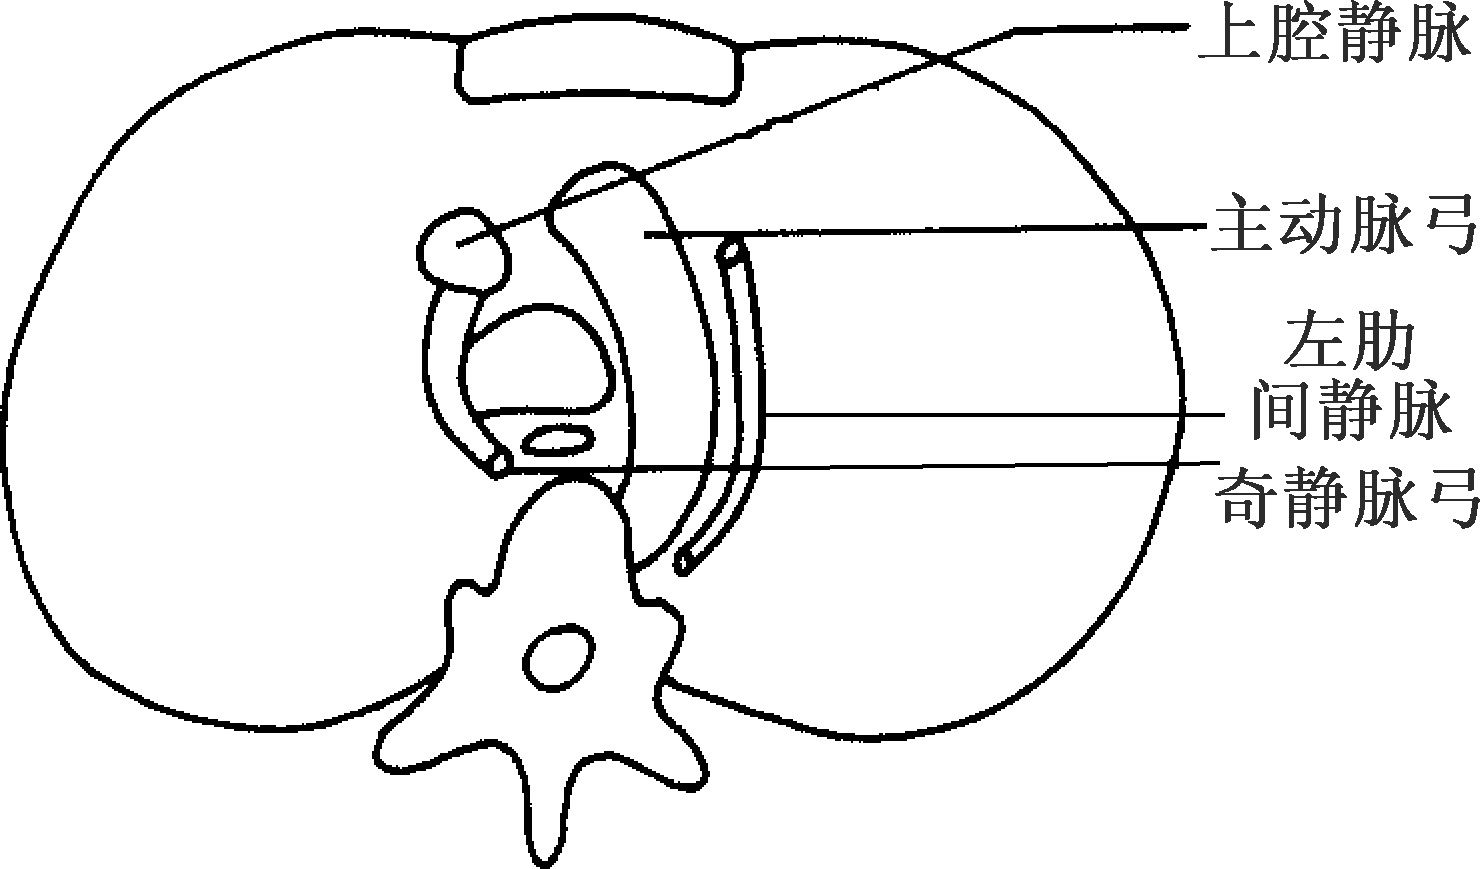
\includegraphics[width=.7\textwidth,height=\textheight,keepaspectratio]{./images/Image00260.jpg}
 \captionsetup{justification=centering}
 \caption{左上肋间静脉环绕主动脉弓}
 \label{fig10-1}
  \end{figure} 

4.主动脉弓下方4cm层面:升主动脉根部位于中央,左心房位于心脏后方,右心房位于升主动脉右侧,右心室流出道位于升主动脉根部左前方,降主动脉位于脊椎左侧。

5.主动脉弓下方7cm层面:主动脉根部及4个房室均显示。主动脉根部在中央,左心房在其后方,右心房在右侧,右心室在前方,左心室在左后方,降主动脉位于脊柱左侧。

6.心室平面:显示左、右心室。左心室在右心室的左后方,降主动脉位于脊柱左侧。

\subsection{心包的CT表现}

在脏层心包(心外膜)下、心脏表面丰富的脂肪组织和纵隔脂肪组织的衬托下,心包可显示得十分清楚,呈一光滑的细线影,厚度多为1~2mm,最厚不超过3mm。右心室前缘处接近膈中心腱区,心包可较厚。一般来说,腹侧心包由于脂肪层较厚而显得较清晰,而某些部位(如左心室侧壁处)由于脂肪少而显示不清。

\section{胸部大血管的先天异常}

\subsection{迷走右锁骨下动脉}

本病是最常见的主动脉弓异常,约占人口的0.5%。

\textbf{【病理】}
这一异常是右锁骨下动脉发自左锁骨下动脉起始部之后的主动脉弓或降主动脉,经食管后方斜行到右侧。

\textbf{【临床表现】}
较少产生临床症状,少数人特别是老年人可产生食管压迫症状,偶尔合并先心病。

\textbf{【CT表现】}
主动脉弓位置稍高于正常人,而且走行接近矢状位与正常的斜行不同。主动脉弓的分支依次是右颈总动脉、左颈总动脉、左锁骨下动脉和右锁骨下动脉。右锁骨下端动脉开口部多扩大为主动脉憩室。右锁骨下动脉在食管和气管后方行走(图\ref{fig10-2})。动态增强扫描有助于确诊。

\begin{figure}[!htbp]
 \centering
 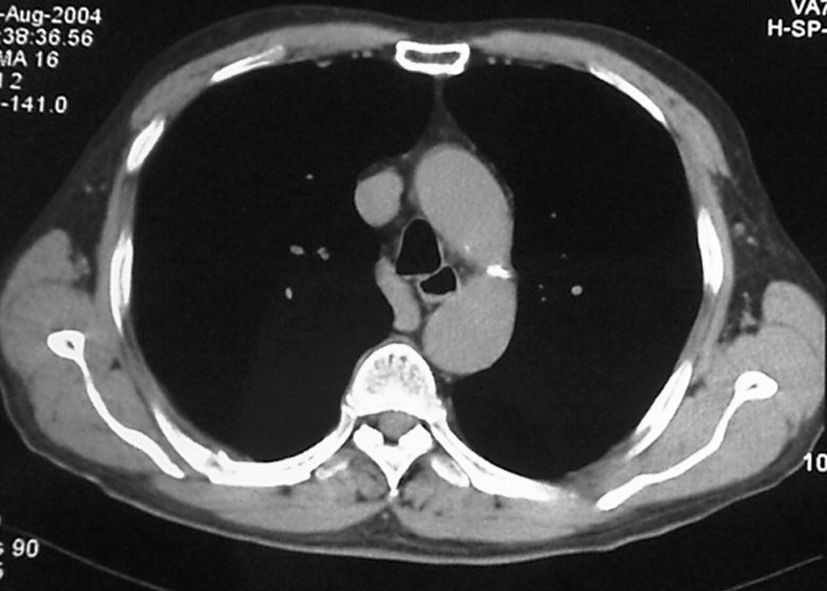
\includegraphics[width=.7\textwidth,height=\textheight,keepaspectratio]{./images/Image00261.jpg}
 \captionsetup{justification=centering}
 \caption{迷走右锁骨下动脉\\{\small 表现为走行于食管、气管右侧的条状高密度灶}}
 \label{fig10-2}
  \end{figure} 

\subsection{左主动脉弓并右降主动脉}

该血管异常少见,且常合并其他血管畸形。胸片及食管造影与双动脉弓或右主动脉弓并迷走左锁骨下动脉有时不易鉴别。

\textbf{【CT表现】}
降主动脉横行于气管、食管后方至脊柱右侧下行,而主动脉弓的几个分支正常。

\subsection{右位主动脉弓}

本病约占0.05%。

\textbf{【病因病理】}
本病是由于左侧第四弓的进化中断而右侧第四弓进化的结果。根据其中断部位,可将右位主动脉弓分为5型。Ⅰ和Ⅱ型:中断部位在左锁骨下动脉远端,为右位主动脉弓伴镜像分支。Ⅲ型:中断部位在左锁骨下动脉与左颈总动脉之间,为右位主动脉弓伴迷走左锁骨下动脉。Ⅳ型:中断部位在左颈总动脉近端,为右位主动脉弓伴迷走无名动脉。Ⅴ型:中断部位在左锁骨下动脉远端与左颈总动脉近端(Ⅰ型+Ⅳ型),产生孤立性左锁骨下动脉,它通过左侧动脉导管与左肺动脉连接。其中以Ⅲ型和Ⅰ型常见,尤以Ⅲ型最常见。

\textbf{【临床表现】} 大多无症状,合并先心病者有相应症状。

\textbf{【CT表现】}
①镜像分支:主动脉弓位于气管和食管右侧,位置通常较高,左无名动脉是第一分支,其次是右颈总动脉、右锁骨下动脉。本型多伴先心病如Fallot四联症等。②伴迷走左锁骨下动脉者:胸片及食管造影与双主动脉弓可不易区别。CT表现主动脉弓位于气管和食管右侧。其弓上有4个分支,从主动脉弓近端至远端的排列顺序是左颈总动脉、右颈总动脉、右锁骨下动脉及左锁骨下动脉。左锁骨下动脉起始部常较膨大形成憩室,从食管、气管后方走行到左侧。

\subsection{双主动脉弓}

\textbf{【病因病理】}
本病是由于胚胎发育过程中两侧第四弓均不退化中断的结果。这两个主动脉弓在气管及食管的两侧汇合于其后方形成降主动脉,通常在左侧下降。每个弓各自发出颈总动脉和锁骨下动脉,极少合并先心病。

\textbf{【临床表现】} 多在1岁内出现气短、复发性呼吸道感染和吞咽困难。

\textbf{【CT表现】}
可显示双侧主动脉弓,它们可以对称,也可不对称,常为右弓大于左弓。在主动脉弓水平上方层面可见各自发出的两根动脉;在主动脉弓水平以下层面显示双侧主动脉弓汇合于食管后方形成降主动脉,还可显示气管受压狭窄的表现。少数病例左主动脉弓闭锁或极小时,CT与右主动脉弓并迷走左锁骨下动脉的鉴别困难。

\subsection{颈位主动脉弓}

本病是一种罕见的血管畸形,它是主动脉弓离开原来的位置,向上延伸至胸廓入口甚至达颈部。

\textbf{【临床表现】} 一般无症状,可出现吞咽困难及呼吸道症状。

\textbf{【CT表现】}
主动脉顶部大约位于颈底部、锁骨内侧的上方;连续层面观察其一端与升主动脉连接,另一端与降主动脉连接。左颈位主动脉弓位于脊柱左侧,右颈位主动脉弓位于脊柱右侧。其两侧颈总动脉和锁骨下动脉通常分开,直接发自主动脉弓。可有食管、气管受压表现。

\subsection{先天性主动脉褶曲畸形}

此畸形可单独存在或合并其他心血管畸形。主动脉褶曲以峡部即动脉韧带附着处为中心,主动脉弓和降部上段形成略呈“S”形的弯曲变形。与主动脉狭窄不同,褶曲部无明显管腔狭窄,血流易通过,但其形态有相似之处,因此又称为假性主动脉狭窄。

\textbf{【临床表现】}
若单独存在可无任何症状,如合并其他心血管畸形则有相应的症状和体征。

\textbf{【CT表现】}
主动脉褶曲部位管腔略窄,其远、近端可略显扩张,甚至可呈瘤样扩张。主支气管局部略有受压推移。左前斜位重建可见主动脉在峡部向前成角。

\textbf{【鉴别诊断】}
主要与主动脉狭窄鉴别。前者褶曲部管腔可略变细,但无明显狭窄;尤其无肋骨切迹(平片可显示),无锁骨下、内乳、肋间动脉及纵隔血管的侧支循环表现,有助于与主动脉狭窄鉴别。

\subsection{先天性主动脉狭窄}

本病是一种常见的主动脉局限性狭窄、闭塞畸形,约90%以上缩窄发生在左锁骨下动脉开口远端的动脉导管或韧带所在区域(即峡部)。多为局限性狭窄;少数病例狭窄较长,在锁骨下动脉近端或累及开口部。

\textbf{【病理】}
主要改变为中膜变形及内膜增厚,成膜状或嵴状向腔内突出。严重者可仅有一数毫米的小孔,甚至完全闭锁。

1.单纯型:约占70%。缩窄在左锁骨下动脉开口远端的主动脉峡部,病变局限,动脉导管已闭合,无其他重要的心血管畸形。

2.复杂型:约占30%。又分为两个亚型:①甲型:在锁骨下动脉开口近端主动脉弓部,或缩窄同时累及左锁骨下动脉开口部或其远端的主动脉,病变较长,可合并迷走右锁骨下动脉。②乙型:约占4/5。合并动脉导管未闭、室缺等。故甲型两上肢血压可不等,只有单侧肋骨切迹,乙型则常有左向右分流征象。

\textbf{【临床表现】}
单纯型狭窄尤其是轻症者,儿童期可无症状,至青少年甚至成年时始出现高血压及心脏症状。病人诉头痛、头晕、气急、心悸及下肢无力、冷及麻木感等。上肢高血压和下肢低血压或无血压、下肢动脉搏动减弱或扪不清为其典型体征。如两上肢血压不等,则应想到为复杂型缩窄。心前区、背部肩胛区常可听到收缩期杂音或血管杂音。重度狭窄或(和)合并粗大动脉导管未闭、室缺者常于婴幼儿期发生心力衰竭。

\textbf{【CT表现】}
应常规增强扫描检查。CT可显示:主动脉狭窄的部位、程度和范围,以及狭窄后扩张和左锁骨下动脉近端扩张,尤其对广泛型狭窄显示较好。但局限型狭窄,特别是蹼状型狭窄且狭窄后扩张不明显时,可呈假阴性。还可显示扩张的内乳动脉及椎旁、肩胛部等处杂乱的侧支循环。三维重建(MPR、SSD),尤其是EBCT可更直观的显示狭窄的部位、程度和范围。EBCT还可显示有无动脉导管未闭、室间隔缺损以及主动脉弓发育情况。

\subsection{左上腔静脉}

左上腔静脉是一种较常见的体静脉异常连接,可单独存在或与右上腔静脉同时存在即双上腔静脉。发病率在正常人群中占0.1%~0.3%,而在先心病中可占4%(其中双上腔静脉约占85%)。75%以上双上腔静脉和单纯左上腔静脉无血液动力学异常。左上腔静脉可伴各种先天性心脏病。

\textbf{【病因病理】}
左上腔静脉是由于胚胎时期左前主静脉未能正常退化所致,最常见两侧上腔静脉同时存在。左上腔静脉回流入冠状窦,冠状窦扩大,然后注入右心房,不产生异常血液动力学改变;少数引流入左房而产生临床症状。25%的病例半奇静脉在左主支气管上方注入左上腔静脉,而奇静脉在同一水平注入右上腔静脉。当两侧上腔静脉同时存在时,右侧横径通常与正常相仿(亦可小于正常),而左侧很少大于右侧(与右侧相等或细小)。

\textbf{【临床表现】} 大多无症状,合并先心病者有相应症状。

\textbf{【CT表现】}
在主动脉弓上层面,左上腔静脉位于左颈总动脉外侧、左锁骨下动脉前方;在主动脉弓及其以下层面位于主动脉弓外侧,继续垂直下行位于肺动脉主干的外侧;经左肺门前方,在心房水平走向后内,沿心包后房室沟行走,进入冠状窦。大约65%的左上腔静脉患者,左头臂静脉变细或缺如。右上腔静脉缺如时表现为一血管结构起源于左、右头臂静脉交界处,向下走行于主动脉弓左侧。左臂注射造影剂并同时行动态增强扫描有助于明确诊断,并与主动脉弓旁的增大淋巴结相鉴别。

\subsection{左头臂静脉畸形}

该畸形较上腔静脉畸形少见。大多数畸形的左头臂静脉位于主动脉弓的下方、升主动脉后,故亦称为升主动脉后或主动脉弓下左头臂静脉,少数为双左头臂静脉畸形。此畸形常伴各种先心病,如室间隔缺损、Fallot四联症等。

\textbf{【临床表现】} 大多无症状,合并先心病者有相应症状。

\textbf{【CT表现】}
①异常的左头臂静脉走行在主动脉弓外侧,在主动脉弓的下方,向右进入主肺动脉窗,走行于气管和升主动脉之间,在奇静脉进入上腔静脉的同一水平或略低水平进入上腔静脉。②双左头臂静脉分为上支和下支,上支多与正常人一样,在正常位置即主动脉弓的前方向右汇入右上腔静脉;而下支则与上述一样经主动脉弓下行走于气管和升主动脉之间,最终汇入上腔静脉。

\textbf{【鉴别诊断】}
①异常的左头臂静脉在主动脉弓及弓上层面与左上腔静脉CT表现相似,但不继续下行,而是进入主肺动脉窗,向右汇入上腔静脉;而左上腔静脉则汇入冠状窦。故高质量的左上臂静脉团注造影剂并快速动态扫描能清晰显示两者血管行程的差别。②不要把左头臂静脉误认为高位右肺动脉。

\section{大血管病变}

\subsection{无名动脉迂曲}

本病又称为无名动脉瘤样迂曲,是较常见的一种异常改变。无名动脉长约5cm,其一端被主动脉弓所固定,另一端被颈部软组织所固定。当发生动脉硬化或高血压时,主动脉扩张伸展,主动脉弓和无名动脉向头侧抬高,由于其上方固定,以至无名动脉弯曲,构成了右上纵隔的边界。

\textbf{【临床表现】}
绝大多数见于50岁以上。多无症状,偶尔压迫邻近组织器官而产生相应症状。

\textbf{【CT表现】}
能清楚地显示无名动脉的走行异常和是否合并动脉瘤。国内有学者将其分为3种类型。①第一型:无名动脉的主动脉开口上方有一短的上升段后,向外呈水平走向,再上升到远端分出右锁骨下动脉和右颈总动脉;②第二型:即第一型的水平段向近端弯曲再向上延伸;③第三型:无名动脉极度迂曲,向外向后突入右上肺与纵隔呈岛状连接。总之,一般无需增强扫描即可诊断。无名动脉瘤呈梭形扩张与本病有别。

\subsection{真性主动脉瘤}

主动脉瘤按病理解剖及形态变化可分为真性、假性及夹层动脉瘤3种。

\textbf{【病因】}
真性动脉瘤是由于主动脉疾病引起的永久性扩张。其扩张可以是均匀一致的累及管壁一周(呈梭形),亦可呈囊性仅累及管壁一周的局部(呈囊状)。真性动脉瘤最常见的病因是动脉硬化,其他少见原因包括梅毒性、主动脉壁内壁退化、主动脉炎、细菌性、结核性或先天性等。

\textbf{【病理】}
真性主动脉瘤是主动脉管腔异常扩张,而血管壁仍保持完整。由于动脉中层弹力纤维破坏,被纤维组织所代替,使管壁变薄而失去弹性,在血流冲击下,向外膨出形成动脉瘤。主动脉粥样硬化性主动脉瘤主要发生于主动脉弓和降主动脉处;细菌性和先天性可累及主动脉窦;梅毒性主要累及升主动脉和主动脉弓。

当瘤体直径在5~10cm时,破裂的危险性为10%;但其直径>10cm时,破裂的可能性达50%。一般主张胸主动脉瘤直径>7cm者行手术治疗。

\textbf{【临床表现】}
胸主动脉瘤的临床表现:一般发病缓慢,瘤体较小者可无自觉症状。瘤体长大或至后期,常见的症状和体征包括几个方面。①疼痛:常为胸背痛,多为隐痛、胀闷痛、酸痛等,可持续存在或为阵发性突然胸痛。撕裂样或刺割样疼痛,并可向一定部位放射为夹层动脉瘤及动脉瘤穿破的重要指征。②呼吸道症状:以气短、咳嗽为常见。③压迫症状:声音嘶哑、吞咽困难、咯血或呕血和颈静脉怒张等。这些症状虽不常见,但为反映瘤体较大或穿破的重要指征。④体表的异常搏动:为晚期主动脉瘤外穿的表现。局部有收缩期震颤及血管杂音,对诊断有较大帮助。

\textbf{【CT表现】}

1.主动脉管腔的局部增粗和变形:管腔局部扩大,升主动脉直径>4.5cm,主动脉弓及降主动脉(胸、腹主动脉)直径>4cm,或与邻近主动脉管径相比超过1/3,可诊为主动脉瘤。如局部囊状扩张时,即使直径小于上述径线也可认为异常(图\ref{fig10-3})。

\begin{figure}[!htbp]
 \centering
 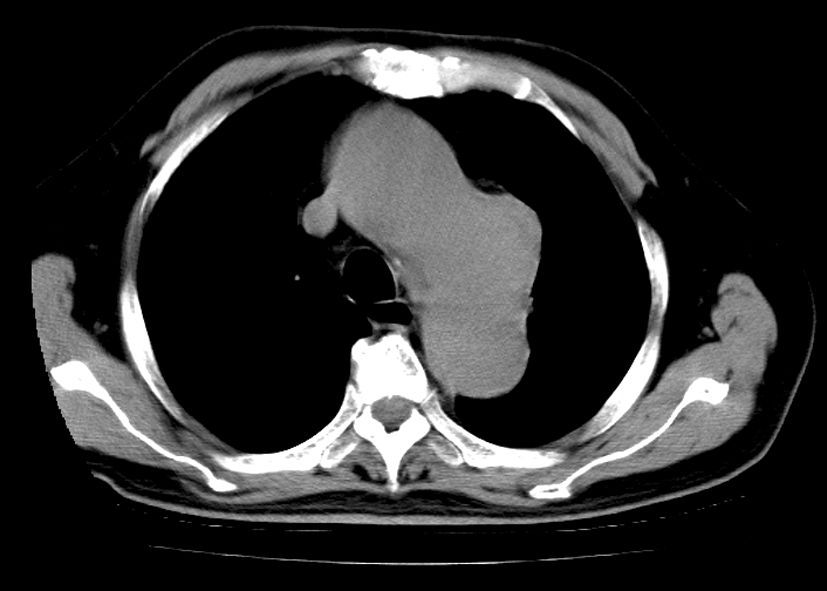
\includegraphics[width=.7\textwidth,height=\textheight,keepaspectratio]{./images/Image00262.jpg}
 \captionsetup{justification=centering}
 \caption{胸主动脉瘤\\{\small 显示主动脉弓局部扩张}}
 \label{fig10-3}
  \end{figure} 

2.周围性钙化:正常主动脉壁厚度为2~3mm,真性动脉瘤的动脉内膜粥样硬化为周围性钙化,这一征象有助于与主动脉夹层相鉴别。

3.附壁血栓形成:常见,呈新月形、半月形或环形等(图\ref{fig10-4})。平扫略低于主动脉内血液。血栓内可有不规则斑块状、斑片状钙化。增强扫描有助于血栓的显示。

\begin{figure}[!htbp]
 \centering
 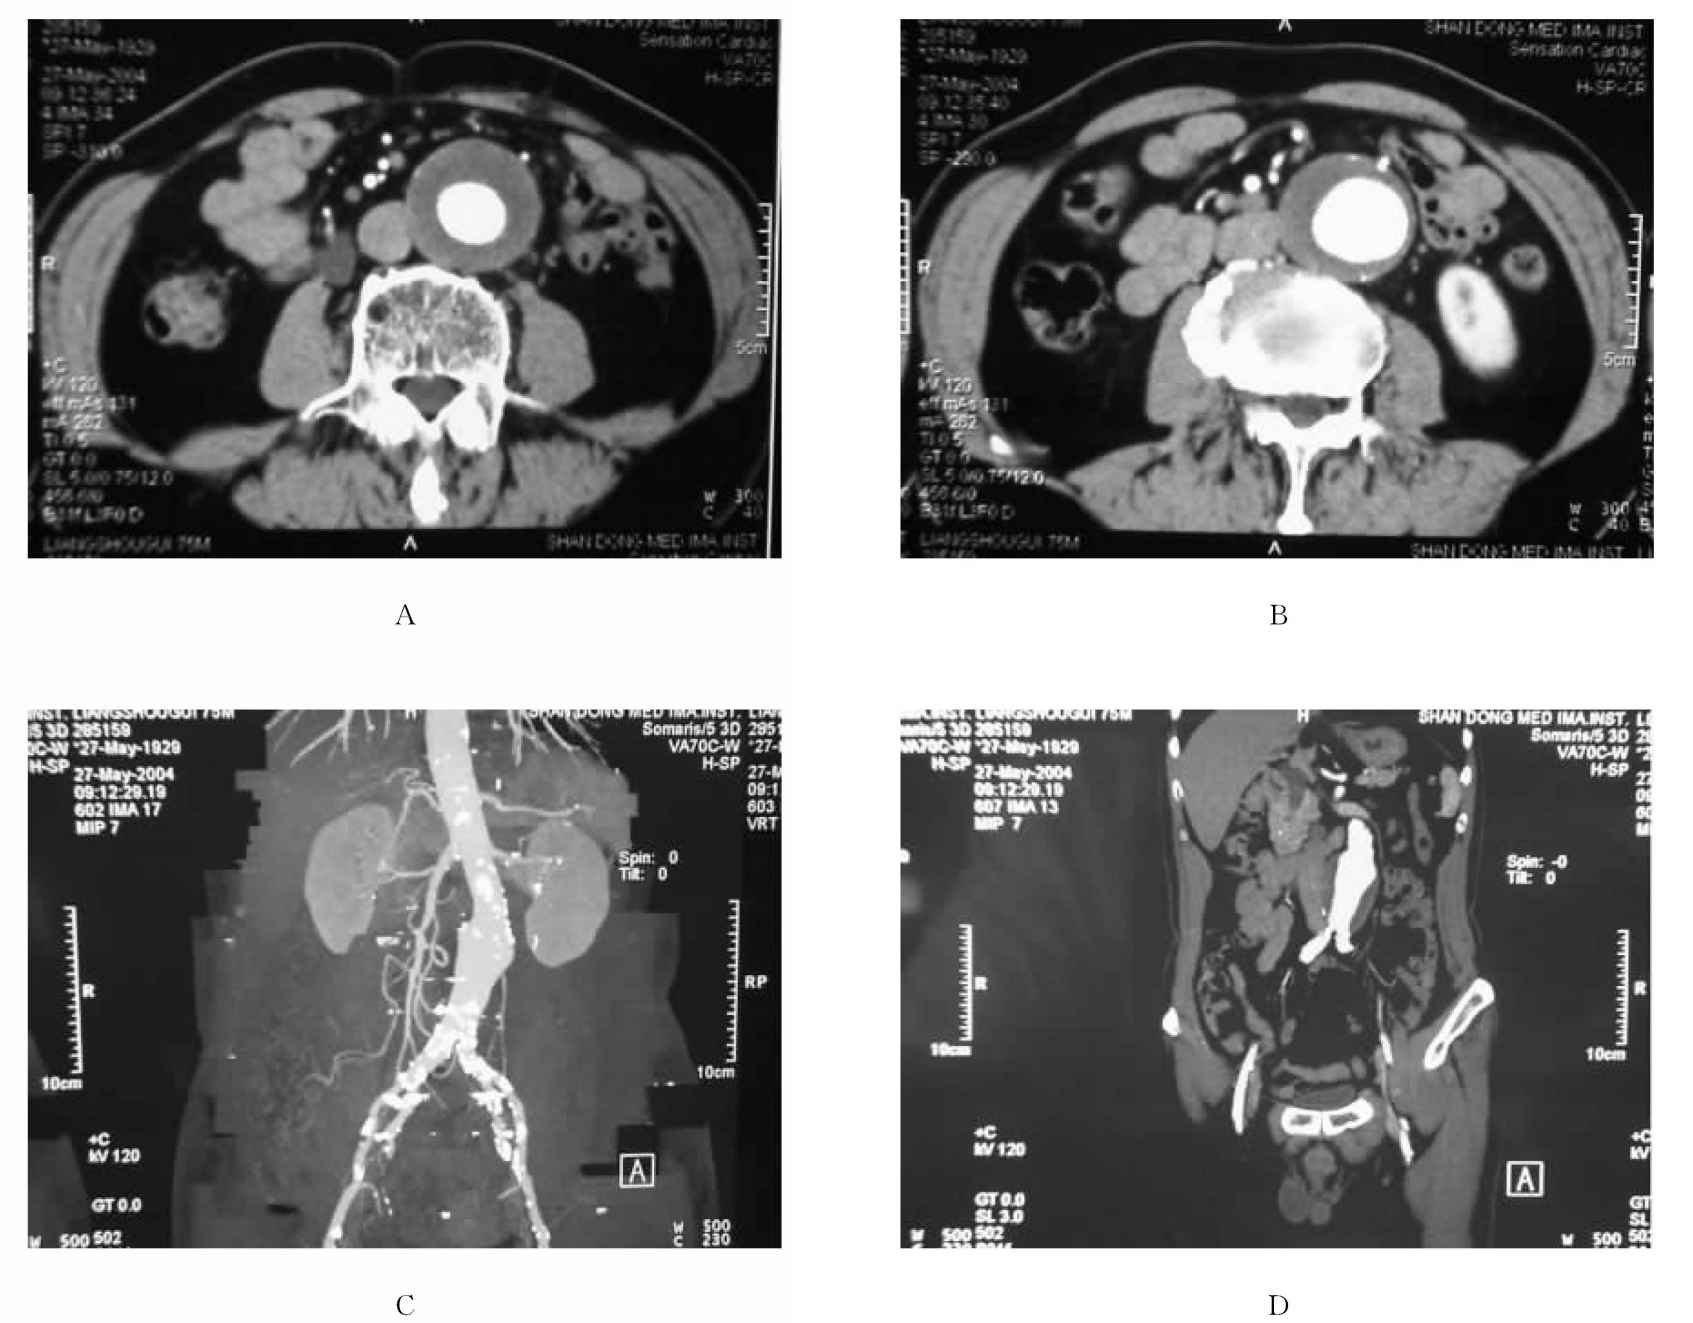
\includegraphics[width=.7\textwidth,height=\textheight,keepaspectratio]{./images/Image00263.jpg}
 \captionsetup{justification=centering}
 \caption{腹主动脉瘤\\{\small 腹主动脉局限增粗,增强扫描可见呈低密度的环状附壁血栓}}
 \label{fig10-4}
  \end{figure} 

4.主动脉瘤与周围脏器的关系:当主动脉瘤增大到一定程度,可压迫推移周围脏器。

5.主动脉瘤渗漏或破入周围脏器:可显示纵隔血肿、主动脉瘤边缘模糊以及胸腔积液等。增强扫描可显示造影剂外渗,但并不常见。有学者认为,主动脉直径>6cm,且瘤壁边缘不整齐、局部变薄、广泛钙化或有造影剂外渗现象,则主动脉瘤有近期破裂危险。

\textbf{【鉴别诊断】}

1.正常主动脉扩张:是由于主动脉压力增高或异常容量负荷引起的暂时性扩张,最常见的原因是高血压。CT显示主动脉扩张通常不伴主动脉壁钙化和腔内血栓形成,扩张非局限性。当整个主动脉极度扩张和迂曲可视为一长纺锤形主动脉瘤。

2.主动脉狭窄、主动脉瓣狭窄:亦可导致狭窄后主动脉局限扩张,结合其他临床及影像学表现可予鉴别。主动脉瓣关闭不全可致主动脉伸展迂曲,但扩张少见。

3.纵隔或纵隔旁肿块:囊性主动脉瘤需注意与其相鉴别。囊性主动脉瘤的囊壁常可见钙化,与主动脉的分界不清而外缘光滑。增强扫描可显示主动脉瘤腔强化与主动脉一致,而其内的血栓不强化;纵隔肿瘤多呈中度强化。

\subsection{主动脉夹层}

本病是主动脉最常见的危重性疾病,发病后48h病死率达36%~71%,合并器官缺血者的病死率达60%。

\textbf{【病因病理】}
90%病例伴高血压和动脉粥样硬化。40岁以下年轻患者多见于主动脉囊性中层坏死(伴或不伴Marfan综合征)。本病亦可见于主动脉瓣二叶式或单瓣畸形、主动脉狭窄和妊娠等。此外,外伤和医源性损伤也是原因之一。

上述病因引起主动脉的同心或偏心性扩张,导致主动脉内膜撕裂,内膜破裂后,血液进入主动脉中层的中1/3与外1/3之间,形成血肿或假性通道,故它不是真正的主动脉瘤。常见的撕裂部位即入口点在主动瓣上方的近端主动脉(4cm以内)或主动脉峡部;在远端可有一个继发撕裂,即出口点;亦可多处破口;形成真假两腔,夹层管道趋向螺旋形。夹层可累及分支如主动脉弓分支、肾动脉和髂动脉。De
Ba
Key等于1965年将其分为3型。Ⅰ型:夹层起源于主动脉近端,累及主动脉弓及降主动脉;Ⅱ型:夹层起源于升主动脉,终止于无名动脉,即仅累及升主动脉;Ⅲ型:夹层起自主动脉峡部,仅累及降主动脉,可伸展到腹主动脉。

\textbf{【临床表现】}
多见于40岁以上男性,40岁以下多见于囊性中层坏死者。按发病情况有急性和慢性(以起病两周为界)之分。多起病急,最常见的症状是胸背部撕裂痛,疼痛可向下延及腹部。部分病人可无症状和症状模糊,其他主要是压迫上腔静脉、喉返神经、食管而出现相应症状。

对突发的非心性和非胸膜性胸痛一般多首先考虑主动脉夹层,其次为急性主动脉壁间血肿、漏血的主动脉瘤、主动脉硬化性溃疡(穿通性)、心包炎、肺动脉栓塞、纵隔血肿等。

\textbf{【CT表现】}
包括直接征象和间接征象两大类。其直接征象即夹层内膜片和真假两腔的显示是本病的特征性表现。多层螺旋CT对主动脉夹层的显示更为清晰。

1.直接征象:①夹层内膜片显示:平扫偶可发现,呈线样稍低密度影,偶可呈稍高密度。增强扫描表现为位于真假两腔之间的线样低密度影。②真假两腔的显示:增强扫描大多数真腔密度明显高于假腔,且假腔峰值出现迟。假腔的形态可呈半球形、新月形、环绕形和不规则形。但也有内膜撕裂口较大时,增强扫描假腔显影相对较快。③内膜破裂口:通常以近端多见,表现为真腔靠假腔侧尖角样突起或内膜片部分、完全中断。

2.间接征象:①钙化内膜内移:即平扫示钙化内膜从主动脉壁外缘内移5mm以上(图\ref{fig10-5})。但真性主动脉瘤内血栓钙化或主动脉周围血肿亦偶可出现类似表现。②主动脉不同程度的迂曲扩张:主动脉各段管径粗细不均且不成比例,多与夹层发生的部位相一致。③腔内血栓:多见于假腔,偶尔假腔完全充满血栓造成诊断困难。④真腔受压变形:真假两腔的大小无一定规律,但通常真腔小于假腔。⑤慢性夹层者偶见其假腔的周围性钙化。⑥并发症:渗漏和破裂,造成心包、纵隔和胸腔积液或积血。国外有文献报道急性者心包积血主要分布于前心包腔、心包上隐窝及横窦,可能与出血部位在心包上方的大动脉周围有关。

\begin{figure}[!htbp]
 \centering
 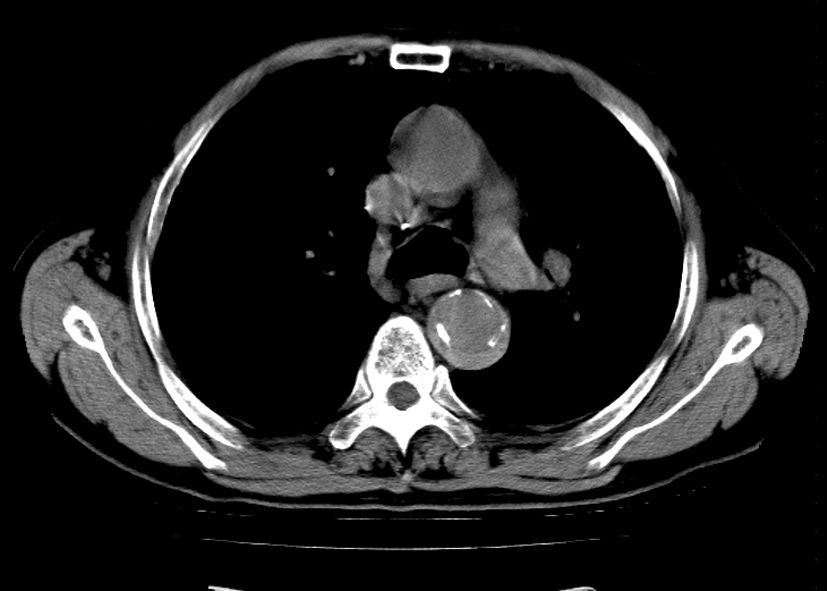
\includegraphics[width=.7\textwidth,height=\textheight,keepaspectratio]{./images/Image00264.jpg}
 \captionsetup{justification=centering}
 \caption{主动脉夹层\\{\small 钙化内膜从主动脉壁外缘内移5mm以上}}
 \label{fig10-5}
  \end{figure} 

3.真、假腔的鉴别:①增强扫描时间-密度曲线通常显示假腔的强化与排空比真腔迟,且密度低;②国外有文献报道团注增强扫描出现鸟嘴样或蛛网状强化均见于假腔;③腔内血栓通常出现在假腔,少数出现于真腔,增强扫描时血栓不强化;④真腔径线通常小于假腔(但并非绝对)且变扁;⑤内膜瓣多平直或突向假腔,少数突向真腔或呈“S”型;⑥如一个腔包绕另一个腔,则被包绕的是真腔,偶可看到3个腔;⑦假腔在升主动脉通常位于前方,而在降主动脉通常位于后方。

\textbf{【鉴别诊断】}

1.伪影:①条形伪影:可酷似撕裂的内膜片,后者为一层薄而弯曲的线样结构;而条形伪影则表现为较粗的直线影,在不同的CT层面上其方向可以不同,特别是伪影常伸展超出主动脉的边缘更具鉴别意义。②升主动脉运动伪影:主要见于螺旋CT扫描,表现为主动脉壁内弧线状界面或类似夹层动脉瘤的假内膜片。伪影多发生于升主动脉近端,以左前方多见。此伪影与升主动脉在收缩期和舒张期不同直径有关。螺旋CT的1s采集时间与平均心动周期(约800ms)相似,而普通CT采集时间长,升主动脉的活动被平均了,故普通CT不易显示。

2.主动脉窦:在主动脉根部CT平扫时,主动脉窦呈3个大小相等的弧形结构,而内膜片仅为1个弧线形结构,同时观察邻近层面不难鉴别。

3.真性主动脉瘤:主动脉夹层不典型者,如假腔内充满血栓而不显影时,常造成诊断困难,但这种情况少见。如见到钙化内膜内移及残留的管腔狭窄或变形,则强烈提示主动脉夹层;而单个扩大的主动脉管腔伴周围性钙化,则是动脉粥样硬化性主动脉瘤的特征。

\subsection{主动脉壁内血肿}

本病又称不典型主动脉夹层,是指主动脉内膜破溃或溃疡,血液在主动脉中层形成血肿;另一种情况是主动脉中膜或外膜的滋养血管破裂出血而形成壁内血肿。占主动脉夹层的5%~20%。其临床表现和治疗方案与典型主动脉夹层相似。

\textbf{【病因病理】}
本病主要与高血压、主动脉粥样硬化、累及主动脉的某些结缔组织疾病或遗传性疾病(如Marfan综合征等)有关。在主动脉粥样硬化斑块的侵蚀、主动脉粥样硬化溃疡形成或者主动脉中层弹性纤维及平滑肌细胞退行性改变的基础上,由于高血压等促发因素的存在,主动脉中层分离而形成假腔。胸部钝伤所致的主动脉中层滋养血管被损伤,亦可并发破裂出血而导致本病。少数真腔与假腔之间有交通,即内膜片上有渗漏孔。

血肿一方面可逐渐吸收,假腔逐渐缩小甚至消失;也可向真腔穿破而演变为主动脉夹层。还可逆行扩展致心包积血、主动脉瓣关闭不全,少数可合并胸腔积血、纵隔血肿或假性动脉瘤。

\textbf{【临床表现】}
与典型主动脉夹层相似。多起病急,最常见的症状是突发胸背部撕裂痛,向肩背部或腹部放射。还有学者报道1例以意识障碍为首发症状。

\textbf{【CT表现】}

1.直接征象:主动脉管壁呈新月状、半月形或环状增厚≥5mm,可达20mm余;该增厚的主动脉壁即假腔的密度,可高于、等于或低于主动脉真腔。增强扫描无内膜破裂形成的双腔主动脉征象,即血肿无强化。病变范围可局限,亦可累及主动脉管壁全程。还可见内膜的钙化移位。治疗后血肿吸收、变小或发展为典型的主动脉夹层。可因血液经血管壁外渗而并发胸腔、心包积液。

2.间接征象:病变主动脉大小、形态变化相对较小;主动脉管腔(真腔)多保持正常,亦可轻度受压;部分病例亦可因主动脉管壁变薄而有所扩张。主动脉粥样硬化斑块穿通溃疡形成时,表现为溃疡呈向腔外突出的龛影;溃疡范围大时可使管腔呈动脉瘤样扩张,但少见。

\textbf{【鉴别诊断】}
①典型主动脉夹层:主动脉壁内血肿无撕裂内膜片,增强扫描无真、假腔形成。但有时与内膜破口封闭、假腔已由血栓充填的慢性主动脉夹层鉴别困难。如主动脉壁内血肿的内膜有渗漏口(通常很小),假腔血流停滞或流动缓慢;而主动脉夹层假腔血流速度快。②大动脉炎:受累主动脉呈较均匀规整的环形增厚,增强扫描呈“双环”征;常累及主动脉的主要分支并导致其狭窄或闭塞。③主动脉粥样硬化斑块:管壁增厚不规则,硬化斑块密度较血液略低,其钙化向腔内移位一般<5mm。④主动脉瘤伴附壁血栓:病变部位呈瘤样扩张,而主动脉壁内血肿伴瘤样扩张者相对少见。⑤纵隔血肿:创伤所致的主动脉壁内血肿应与其鉴别。前者主动脉腔(真腔)一般有变形,内径正常或缩小;而纵隔血肿一般无此征象。

\subsection{假性主动脉瘤}

动脉血管壁因某种原因破裂后形成局部血肿,当血肿表层的机化形成纤维组织囊壁,并且囊腔与管腔相通时,称为假性动脉瘤。

\textbf{【病因病理】}
常见病因的有外伤和心脏血管术后,此外胰腺炎、白塞氏综合征、动脉硬化等也可引起本病。瘤壁主要由纤维组织构成,而不是动脉壁结构。

\textbf{【临床表现】}
临床多有诱因,如外伤、手术或发热史。可发生在外伤或手术后数月、数年甚至数十年。发病时有剧烈疼痛等症状。

\textbf{【CT表现】}
外伤所致者好发于主动脉弓降部、动脉导管韧带及左锁骨下动脉开口附近。平扫肿块与主动脉关系密切,在慢性病例瘤壁和瘤腔内常有斑块状钙化。增强和延迟扫描见瘤腔的显影和排空均较主动脉迟;瘤腔与主动脉之间有颈相连;瘤腔内常有血栓存在,甚至可完全被血栓充填,而误为软组织肿块。慢性病例瘤壁钙化和强化常见;而急性病例则无;亚急性病例瘤壁可强化,而钙化少见。主动脉假性动脉瘤可压迫邻近器官。

\subsection{Marfan综合征}

本病是一种常染色体显性遗传性结缔组织疾病,多见于青壮年。典型者包括下列3方面:①肌肉骨骼系统:表现为肢体细长、蜘蛛指趾、韧带松弛、脊柱侧弯以及漏斗胸等;②眼:晶体脱位或半脱位为其典型变化,临床表现高度近视;③心血管系统:升主动脉扩张或主动脉瘤形成(主要累及升主动脉根部、主动脉瓣环和窦部),可并发主动脉瓣关闭不全或主动脉夹层。

\textbf{【病理】}
本病在心血管系统的病理基础是主动脉中层囊性坏死。主动脉瓣环的扩大、窦瘤或升主动脉夹层可引起或加重主动脉瓣关闭不全。

\textbf{【临床表现】}
本病多见于青壮年。典型者有上述肌肉骨骼、眼和心血管系统改变。只有心血管系统改变者称为心血管型马凡综合征。临床表现取决于有无主动脉瓣关闭不全及其程度,严重者引起左心衰竭,部分有心绞痛症状,升主动脉瘤样扩张可无症状。

\textbf{【CT表现】}
主动脉受累者以增强扫描为佳。①主动脉窦及升主动脉根部瘤样扩张:病变累及主动脉窦部及瓣环为其特点,升主动脉远段受累常不严重;②主动脉夹层;③左心室增大;④应注意观察头臂动脉、降主动脉、腹主动脉有否受累。

\subsection{多发性大动脉炎}

本病是一种慢性进行性非特异性大动脉炎。

\textbf{【病因】}
尚不明确。患者发病时血沉增快、免疫球蛋白G增高、类风湿因子阳性和血清中抗主动脉抗体升高等。故本病可能与感染后的自体免疫有关。

\textbf{【病理】}
本病是一种以中膜损害为主的全动脉炎,动脉全层呈弥漫性或不规则增厚和纤维化。增厚的内膜引起管腔狭窄和阻塞。显微镜下中膜有广泛的弹力纤维和平滑肌断裂、破坏以及炎性细胞浸润、肉芽组织增生,少数可形成动脉瘤。

可将本病分为4型。Ⅰ型:病变主要累及主动脉弓及其分支;Ⅱ型:病变主要累及胸降主动脉、腹主动脉及其分支;Ⅲ型:常见,为混合型;Ⅳ型:主要累及肺动脉。

\textbf{【临床表现】}
本病好发于青壮年,男女之比约为1∶10,偶见于少年儿童。起病时多有发热、食欲不振、周身不适、体重减轻、胸痛、乏力,以及受累动脉狭窄、阻塞的多种临床表现,如头臂动脉阻塞症状、肾血管性高血压、主动脉缩窄综合征、胸腹主动脉瘤、头臂动脉瘤等。

\textbf{【CT表现】}
①急性期:受累主动脉壁增厚,病变呈连续性侵犯一段主动脉,而非“跳跃式”发展;部分轮廓欠清,为主动脉周围炎所致。而正常主动脉壁除非有贫血存在,一般不能显示。增强扫描血管壁呈“双环征”,内环指主动脉内面因黏液样或凝胶状水肿呈低密度,外环指主动脉中膜和外膜因血管增生等炎性改变而呈高密度强化。②慢性期(或晚期):管壁增厚较急性(活动)期轻,管壁可呈局限斑片状或环状广泛钙化。环状广泛钙化者增强扫描管壁呈多环状,即内膜、外膜呈低密度,而钙化中膜呈高密度;如无钙化或呈少许斑片状钙化,增强扫描则整个管壁呈低密度。③管腔狭窄或增宽:以狭窄多见,可同时显示胸、腹主动脉及其较大分支不同程度的狭窄、阻塞或(和)瘤状扩张同时存在;动脉瘤形成较少见。本病约1/3累及肺动脉,可见受累肺动脉(可涉及肺动脉主干至段肺动脉)狭窄或梗阻、管壁增厚。

\subsection{主动脉瓣钙化}

国外有学者将主动脉瓣钙化程度分为3级:CT上见微小的瓣膜钙化为Ⅰ级;见有中间钙化为Ⅱ级;累及三个瓣前尖的广泛性钙化伴中心聚集≥1cm为Ⅲ级。通过相应超声心动图显示,主动脉瓣钙化约15%有主动脉狭窄。主动脉狭窄者多为Ⅱ级钙化,而Ⅱ级和Ⅲ级钙化者约31%为主动脉狭窄。他们认为CT上发现的主动脉瓣钙化是一种常见的通常无临床意义的所见。

但我们认为对主动脉瓣钙化的病人,尤其老年人,注意综合分析(如有无左室肥大),排除主动脉瓣狭窄即老年人退行性心脏瓣膜病是必要的。

\subsection{上腔静脉综合征}

本病又称上腔静脉阻塞综合征,是由于各种病因引起的完全或不完全性上腔静脉阻塞,导致血液回流受阻,引起一系列临床表现。

\textbf{【病因病理】}
上腔静脉阻塞主要是由恶性肿瘤压迫、直接侵犯或癌栓所致;良性病变主要是纵隔肉芽肿性疾病。病理上上腔静脉完全或不完全性阻塞,其主要侧支循环通路有:奇静脉和半奇静脉、内乳静脉、椎静脉、上腹静脉和侧胸静脉,上肋间静脉和食管旁静脉也可参与部分侧支循环。

\textbf{【临床表现】}
头颈部及上肢水肿,上肢、颈部和胸部可见浅表静脉曲张。如阻塞发展迅速可引起脑水肿而出现相应症状。

\textbf{【CT表现】}
平扫只能显示一些引起上腔静脉阻塞的原因,如肿块、增大的淋巴结、动脉瘤等。偶尔显示奇静脉、半奇静脉扩张。增强扫描可见上腔静脉和(或)其主要分支不显影或见有充盈缺损,以及侧支循环显影。上腔静脉受压和(或)受侵犯,受压表现为管腔明显变形,有时呈裂隙状甚至闭塞;肿瘤侵犯上腔静脉示管腔变窄且不规则。单纯受压移位难以鉴别良恶性,但良性病变造成上腔静脉阻塞的概率很低。

\textbf{【鉴别诊断】}

1.癌栓与血栓:两者多难以鉴别。①平扫:癌栓与周围血液的密度相仿或略低。新鲜血栓密度较高,与周围血液相近;而陈旧性血栓密度略低。②增强扫描:均呈低密度充盈缺损。癌栓有时可表现为中心性低密度而周边密度增加的充盈缺损,可能是局部静脉壁的血管增加或肿瘤滋养血管强化所致。癌栓形成患者往往同时可见上腔静脉周围肿块压迫或包绕表现,而血栓形成者多无此表现。

2.层流现象:仰卧位增强扫描早期,可出现上腔静脉后壁下一带状高密度区,而其余部位呈低密度,是由于造影剂比重高于血液向下沉积所致;也可表现为血管周边密度高于中心,此乃造影剂沿管壁流动较慢所致。上述现象即层流现象,应注意与血栓和癌栓相鉴别,该层面重复扫描或延迟扫描即可鉴别。

\subsection{上腔静脉瘤}

先天性上腔静脉瘤非常少见,是因管壁发育不良而扩张所致。

\textbf{【病理】}
管壁结构发育不良,管壁局限性薄弱和扩张。扩张可呈梭形或囊状(憩室样),多发生于奇静脉汇入上腔静脉处。梭形几乎累及上腔静脉全长的90%,囊状可压迫上腔静脉甚至导致上腔静脉阻塞综合征。下腔静脉膈上段静脉瘤十分罕见。

\textbf{【临床表现】}
多无明显症状,常为偶然发现。偶有上腔静脉阻塞综合征。

\textbf{【CT表现】}
CT可清楚显示上腔静脉瘤的类型、大小及有无血栓。上腔静脉瘤的诊断必须是管腔局限扩大,大于邻近管腔的1倍以上,且其大小、形态不受呼吸、体位改变的影响。瘤内常有血栓形成甚至机化。

\textbf{【鉴别诊断】}
应与上腔静脉扩张相鉴别。后者继发于右心梗阻、长期右心或体静脉高压,往往扩张范围较长,常波及下腔静脉,大小、形态随呼吸、体位改变而有所变化,很少有血栓形成。

\subsection{肝内段下腔静脉脂肪沉积}

本病是少见的、临床上无症状的正常组织变异,少数患者该脂肪沉积可能为右肝组织萎缩的表现。

\textbf{【CT表现】}
圆形或椭圆形脂肪密度组织凸入下腔静脉腔内,位于下腔静脉肝内段并邻近下腔静脉内壁,且均可明确显示下腔静脉内壁插入“腔内脂肪”与腔外脂肪之间。国外有学者通过冠状面重建显示,脂肪沉积的“腔内脂肪”与腔外脂肪相连,故认为起源于管腔之外,应属管腔外病变涉及腔内。

\textbf{【鉴别诊断】}
该病可误诊为血栓、原发性肿瘤(如平滑肌肉瘤)、肿瘤转移(如肾、肾上腺恶性肿瘤),但病变呈脂肪密度,不难与上述病变相鉴别。

\section{心脏病变}

\subsection{先天性心脏病}

对先天性心脏病的诊断,目前最常应用的是多普勒心动超声图、心血管造影和胸部平片。其CT诊断价值如下:

1.显示大血管的位置及相互关系:①基本正常:即升主动脉位于肺动脉的右后方,见于正常心脏和Fallot四联症;②主动脉和肺动脉完全并列:可呈左右并列或前后并列,主要见于右心室双出口;③主动脉位于肺动脉的左前方,见于校正型(左襻型)大血管转位;④主动脉位于肺动脉的右前方,见于右襻型大血管转位。

同时,CT还可准确测定大血管的直径,如肺动脉高压可见肺动脉主干直径超过升主动脉直径;原发性肺动脉扩张病例,虽肺动脉干扩张,但周围血管分支无改变。

2.显示内脏位置以及与心脏、大血管的关系:CT易于显示肝脏、脾脏、胃腔以及支气管、肺的形态和脾脏与下腔静脉的位置关系,从而推测左、右心房的位置。如:①无脾综合征:肝脏对称位(或称水平肝)、胃在中线、胰腺可移动、小肠可旋转不完全。双侧支气管都呈右侧型,双肺都为3叶。双侧心房都具有右心房解剖特征。下腔静脉可引入任何一侧心房,但通常都引入肝影相对较大的一侧。多合并右旋心,以及单心房、单心室、肺动脉狭窄或闭锁、完全性肺静脉异位引流、双侧上腔静脉、永存动脉干和大动脉转位等。②多脾综合征:脾脏呈多块状、肝呈对称位、胃位置不定。双侧支气管都呈左支气管型,双肺各为两叶。双心房都具有左心房解剖特征。常见上、下腔静脉畸形,常合并单心房及其他心内畸形。

16层以上螺旋CT、EBCT对先心病的诊断有许多优势,更有利于显示心脏大血管的解剖结构(如心内畸形)、空间位置及连接关系。

\subsection{风湿性心脏病}

本病的活动期心肌、心内膜及心包均可被风湿性炎症所侵及,慢性者主要累及心脏瓣膜。

本病的诊断,常规CT很少应用,但在显示瓣膜的钙化、左心房的血栓形成、肺静脉高压所致广泛间质性改变,以及左房室瓣病变少见的伴随畸形肺静脉曲张等方面具有一定优势。EBCT可观察瓣膜运动情况、测量瓣膜的面积以及分析返流量。

文献报道,CT对左心房血栓尤其左心耳部血栓的检出率高于超声,其特异性也高。左心房血栓大都发生于左心耳部和左心房体上部后侧壁,呈均质低密度充缺或混杂密度的充缺,平扫时可见散在斑点状或层状钙化(图\ref{fig10-6})。有文献认为形态不规则、呈多个尖角状突出的充盈缺损,结合上述的血栓好发部位,是左心房血栓的特征。

\begin{figure}[!htbp]
 \centering
 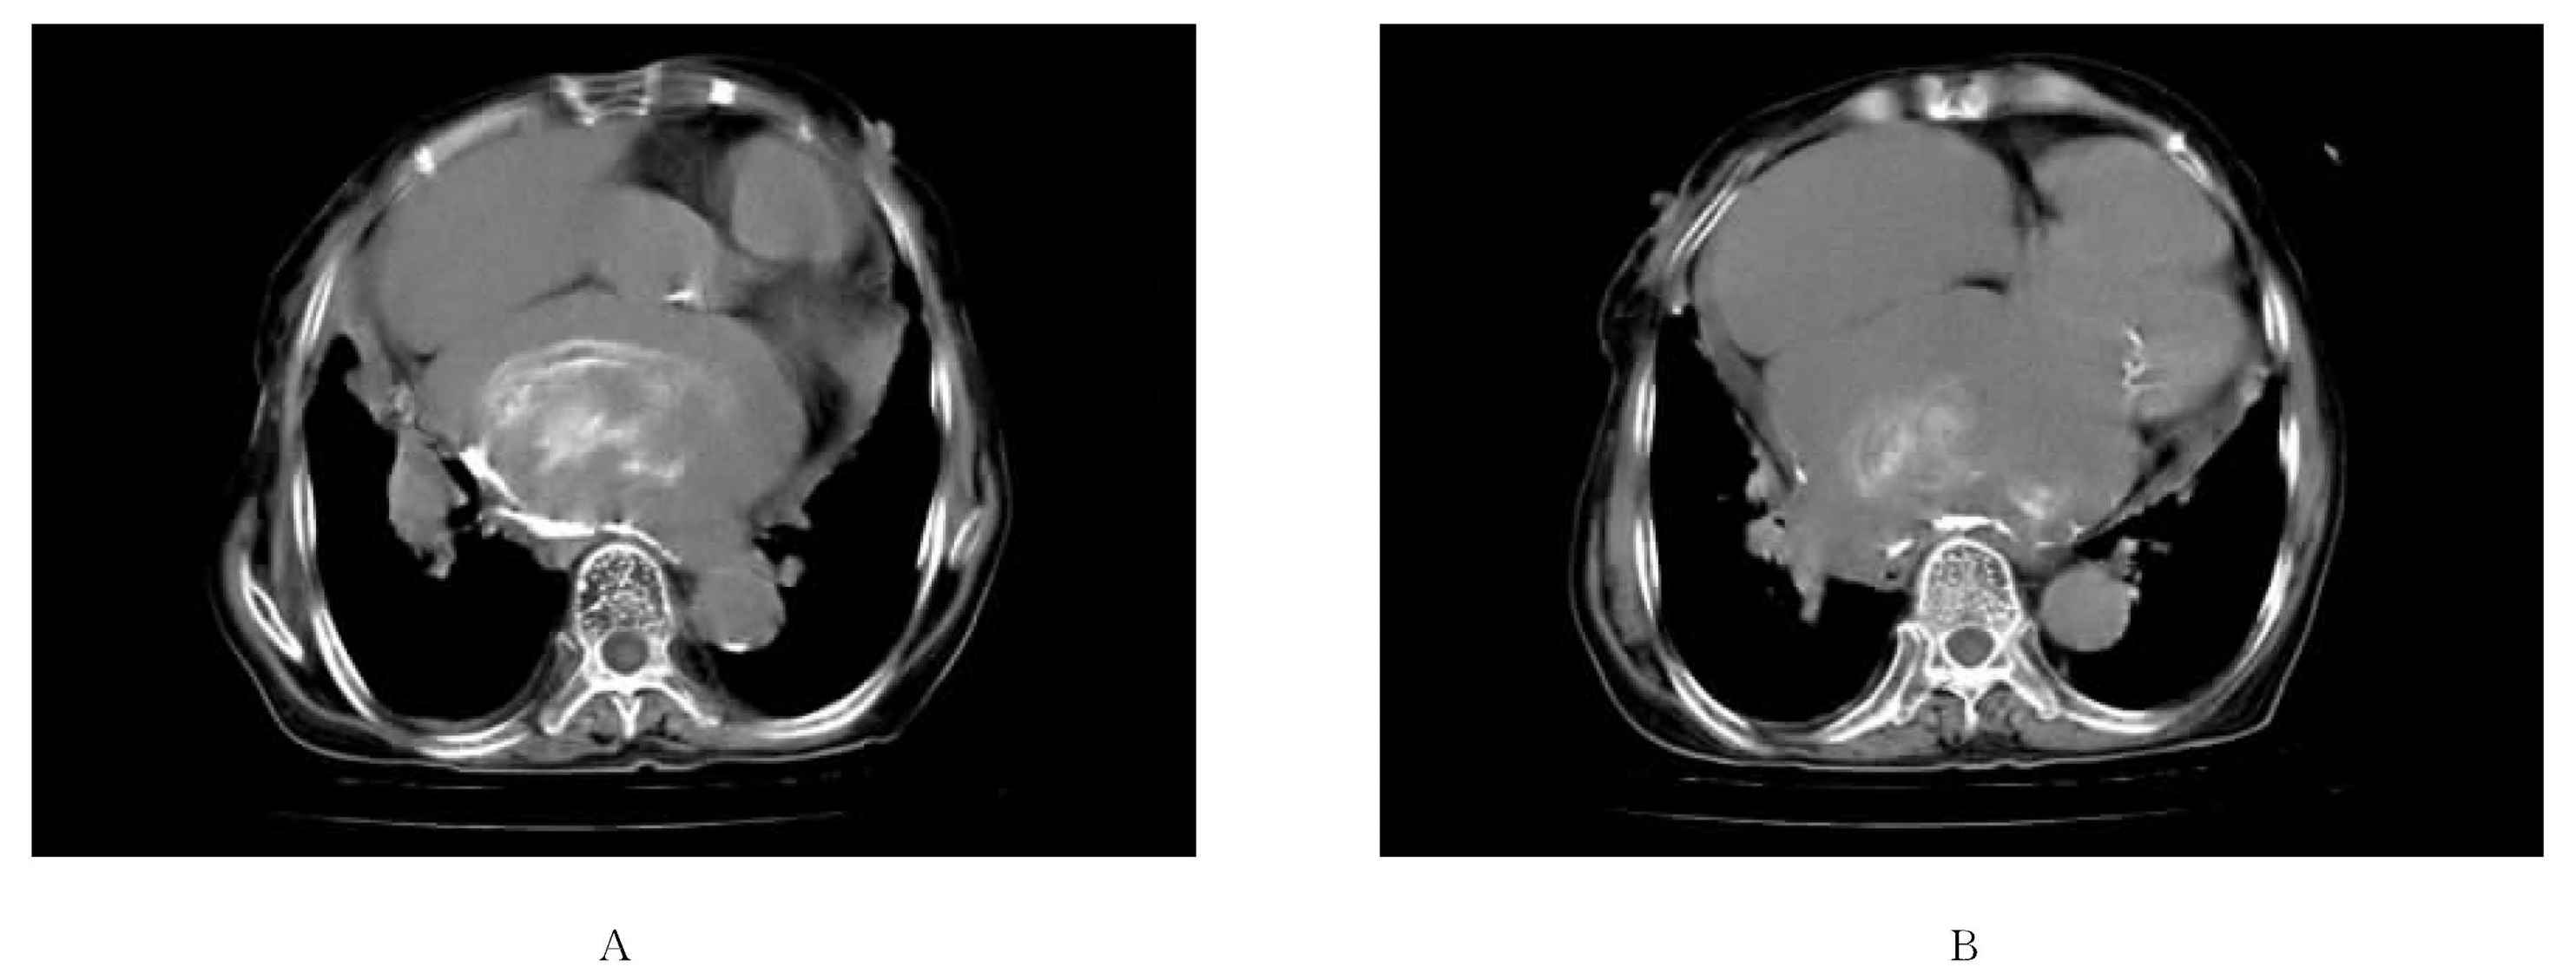
\includegraphics[width=.7\textwidth,height=\textheight,keepaspectratio]{./images/Image00265.jpg}
 \captionsetup{justification=centering}
 \caption{风湿性心脏病\\{\small 左心房血栓内有斑片状和层状钙化}}
 \label{fig10-6}
  \end{figure} 

\subsection{心肌病}

心肌病现在的概念是指原发性心肌病(又称特发性心肌病),即原因不明的心肌疾病,而并非指临床已知病因的心肌损害。常规CT检查对其诊断受到一定限制。

\textbf{【病理】}
可分为以下3类。①扩张型心肌病:占原发性心肌病的70%,左和(或)右心室重度扩张,伴心肌肥厚及心室收缩功能减退。②肥厚型心肌病:占原发性心肌病的20%,以左心室肥厚为主,左心室容量减少。③限制型心肌病:最少见,为心内膜心肌纤维化和嗜酸细胞增多性心内膜心肌病;由于心内膜心肌瘢痕形成,限制了心脏的充盈,病变晚期则发生心腔闭塞。

\textbf{【临床表现】}
常有心悸、气粗、胸痛、眩晕、心律失常及心衰等。有时有胸部压迫感、腹胀、咯血、肺部啰音及肝大、颈静脉怒张等。

\textbf{【CT表现】}
本病的诊断原则是排除继发因素所致的心腔扩大或心肌肥厚,方可做出扩张或肥厚型心肌病的诊断。

1.扩张型心肌病:表现为心腔扩大,主要为心室扩大,心房也可有增大。左心室舒张末期容积增大,超过正常值(116.6±13.6)ml。EBCT见收缩期和舒张期心腔无明显变化,心壁变薄。每搏量降低或正常(约为70~90ml),射血分数明显降低。平扫无冠状动脉钙化灶,而与冠心病有别。

2.肥厚型心肌病:为室间隔不对称性增厚,正常室间隔舒张末期厚为(9.0±1.8)mm。EBCT还可显示左心室游离壁(尤其前壁和侧壁)也增厚,并见肥大的乳头肌。电影扫描心肌增厚率降低(小于30%);动态观察心肌运动功能降低,二尖瓣前叶于收缩期向室间隔方向摆动。平扫亦无冠状动脉钙化灶,而与冠心病有别。

3.限制型心肌病:因主要侵犯心室流入道和心尖造成变形缩窄,而致双心房扩大和下腔静脉扩张。偶可见心包和(或)胸腔积液。电影扫描显示心肌运动顺应性下降,舒张期功能明显受限,心室壁运动明显减弱。心室舒张末期容积减小,每搏量降低,射血分数降低,心肌增厚率降低等。

\textbf{【鉴别诊断】}
①需结合临床与继发性心肌病(感染性、内分泌性、代谢性、中毒、药物过敏、结缔组织病等)、高血压、瓣膜病或先天性心脏病引起的心肌异常病理形态相鉴别。②由于CT可清楚显示心包的厚度和钙化,是鉴别限制型心肌病与缩窄性心包炎的最佳影像学技术之一。两者临床表现相似,CT图像上均可见双房增大和下腔静脉扩张。但前者心包结构正常,后者心包增厚(厚度>3mm)伴或不伴心包钙化。

\subsection{冠状动脉粥样硬化性心脏病}

冠状动脉粥样硬化病变主要累及冠状动脉的大分支和其近端,好发于左前降支近、中1/3,右冠状动脉中1/3,其次为回旋支。常见两支以上的多支病变。

\textbf{【病理】}
冠状动脉粥样硬化有4个阶段。①脂质浸润前期。②脂点、脂纹和粥样斑块形成。③由粥样斑块发展成纤维斑块,此时有钙化发生。④复合性斑块:斑块中央脂质坏死,内膜破溃形成粥样溃疡,血小板聚集,可形成血栓。早期的脂点、脂纹乃至中心斑块可以自然消退,即使形成纤维性斑块也可在一定时期相对稳定。

冠状动脉粥样硬化斑块主要含以下成分:①以平滑肌细胞、巨噬细胞和淋巴细胞为主的细胞成分;②以胆固醇为主的脂质成分(粥样成分);③胶原纤维等细胞外间质成分。动脉粥样硬化斑块破裂及其伴随的血栓形成是引起冠脉狭窄或闭塞的重要病理基础。脂质斑块最易破裂,这种易碎斑块具有斑块内部细胞外胆固醇含量高、脂质核心大、覆盖斑块的纤维帽薄、炎性细胞浸润使纤维帽易损伤的特征。并可呈多灶性。钙化斑块其钙化可位于中心或周边。

冠状动脉狭窄分为4级。Ⅰ级:狭窄在25%以下;Ⅱ级:狭窄在25%~50%;Ⅲ级:狭窄在51%~75%;Ⅳ级:狭窄在76%以上。当狭窄达Ⅲ~Ⅳ级时,冠状动脉的血液供应和心肌耗氧之间失去平衡,产生供血不足,临床出现心绞痛等症状。轻度心肌缺血,心肌细胞出现变性、肿胀,但随着侧支循环的代偿,此时是可逆的。如缺血进一步加重,则心肌细胞可出现缺血性坏死。如坏死仅限于心内膜下,称为心内膜下心肌梗死(非穿壁性心肌梗死);如超过心壁的1/2以上,则称为穿壁性心肌梗死。

\textbf{【CT表现】}

1.冠状动脉粥样硬化斑块的检测

目前的CT技术在对冠状动脉脉粥样硬化斑块的研究中突出表现在两个方面:①对冠脉钙化的检测(见后述);②对软斑块的检测。

早期的MSCT研究,将斑块分为钙化斑块和非钙化性斑块(即软斑块)。近些年来,国外学者将斑块分为3类并分别测量其CT值。①软斑块:CT值分别约(6±28)Hu、(-5±25)Hu、(14±26)Hu不等;②中等斑块:CT值分别约为(83±17)Hu、(51±19)Hu、(91±21)Hu不等;③钙化斑块:CT值分别约(489±372)Hu、(423±111)Hu、(419±194)Hu不等。

国外还有学者总结不同成分斑块的CT值为:新鲜血栓为20Hu,脂质斑块为50Hu,纤维斑块为100Hu,钙化斑块>300Hu。

各家的研究表明,CT可准确地将斑块分型,但还需进一步用MSCT更细致地研究观察斑块的脂核、纤维帽及钙化。而且MSCT空间分辨力尚不够高,部分容积效应影响其密度的测量,以及时间分辨力的限制,影响了其在临床的广泛应用。

2.冠状动脉钙化的检测

冠脉钙化是动脉粥样硬化的标志和早期征象之一,检出钙化意味着粥样硬化斑块的存在。①钙化的阈值(诊断标准):螺旋CT值≥90Hu、EBCT≥130Hu,面积≥1mm\textsuperscript{2}
的病变定为钙化。②钙化的积分:在EBCT或螺旋CT(以多层螺旋CT为优)每一层面上画出所有符合上述钙化病变的兴趣区,自动测量兴趣区的面积(mm\textsuperscript{2}
)和兴趣区内的最大CT值。依据兴趣区内的最大CT值将钙化积分定为1~4(即密度积分系数),1=133~199Hu,2=200~299Hu,3=300~399Hu,4≥400Hu。每一兴趣区的积分值=面积×密度积分系数。所有20层(一般自主肺动脉分叉下缘向下连续扫描20层)的积分之和即为总的钙化积分。③钙化的形态:多表现为依冠脉走行的斑点状、条索影,亦可呈不规则轨道状或整条冠脉钙化。④钙化的部位:按解剖分4组,即左主支、左前降支、旋支、右冠状动脉。对角支的钙化计入左前降支,钝缘支计入旋支。⑤钙化数的计算:尚不统一,以支为单位或以病灶为单位,都有缺点。

临床意义:①一般认为钙化积分越高,则冠脉狭窄的发病率越高。如未发现冠脉钙化,仅5%有冠心病可能。冠脉狭窄Ⅲ级以上者极少不出现钙化。欧美国家中,50岁以上的患者,如钙化积分为0或<10,则冠心病的发病率很低;积分为11~400则提示冠脉狭窄的可能;积分>400一般意味着有冠脉狭窄存在。②但冠脉钙化的存在并非完全等同于冠脉狭窄。有时老年患者由于长期的代偿性血管重建,管腔扩张,虽然出现钙化且积分很高,但冠脉造影并不提示狭窄。③如果年轻患者已有临床症状,而钙化分数诊断准确性并不高,是因病程短暂,无冠脉钙化出现。虽然50岁以下组敏感性低,但特异性高;50岁以上组发现钙化的敏感性高,但特异性低。总之,发现冠脉钙化即表示有粥样硬化存在,但并不一定有>50%(Ⅲ级以上)的狭窄性冠心病的存在。

3.冠心病冠脉CTA的基本征象

①冠脉管腔边缘不规则、半圆形“充盈缺损”和不同程度的向心性狭窄和阻塞,为粥样斑块和管壁增厚的反应。在充盈缺损基础上示有龛影或管腔内透明区、杯口状阻塞、次全阻塞等则为斑块破裂、溃疡和继发血栓形成的反映。重度阻塞和狭窄常为继发性血栓及其后遗病变所致(图\ref{fig10-7})。②冠脉痉挛:多在原有固定狭窄基础上发生,也可见于正常冠脉。③血栓、栓塞和阻塞再通。④冠脉扩张和动脉瘤形成。

\begin{figure}[!htbp]
 \centering
 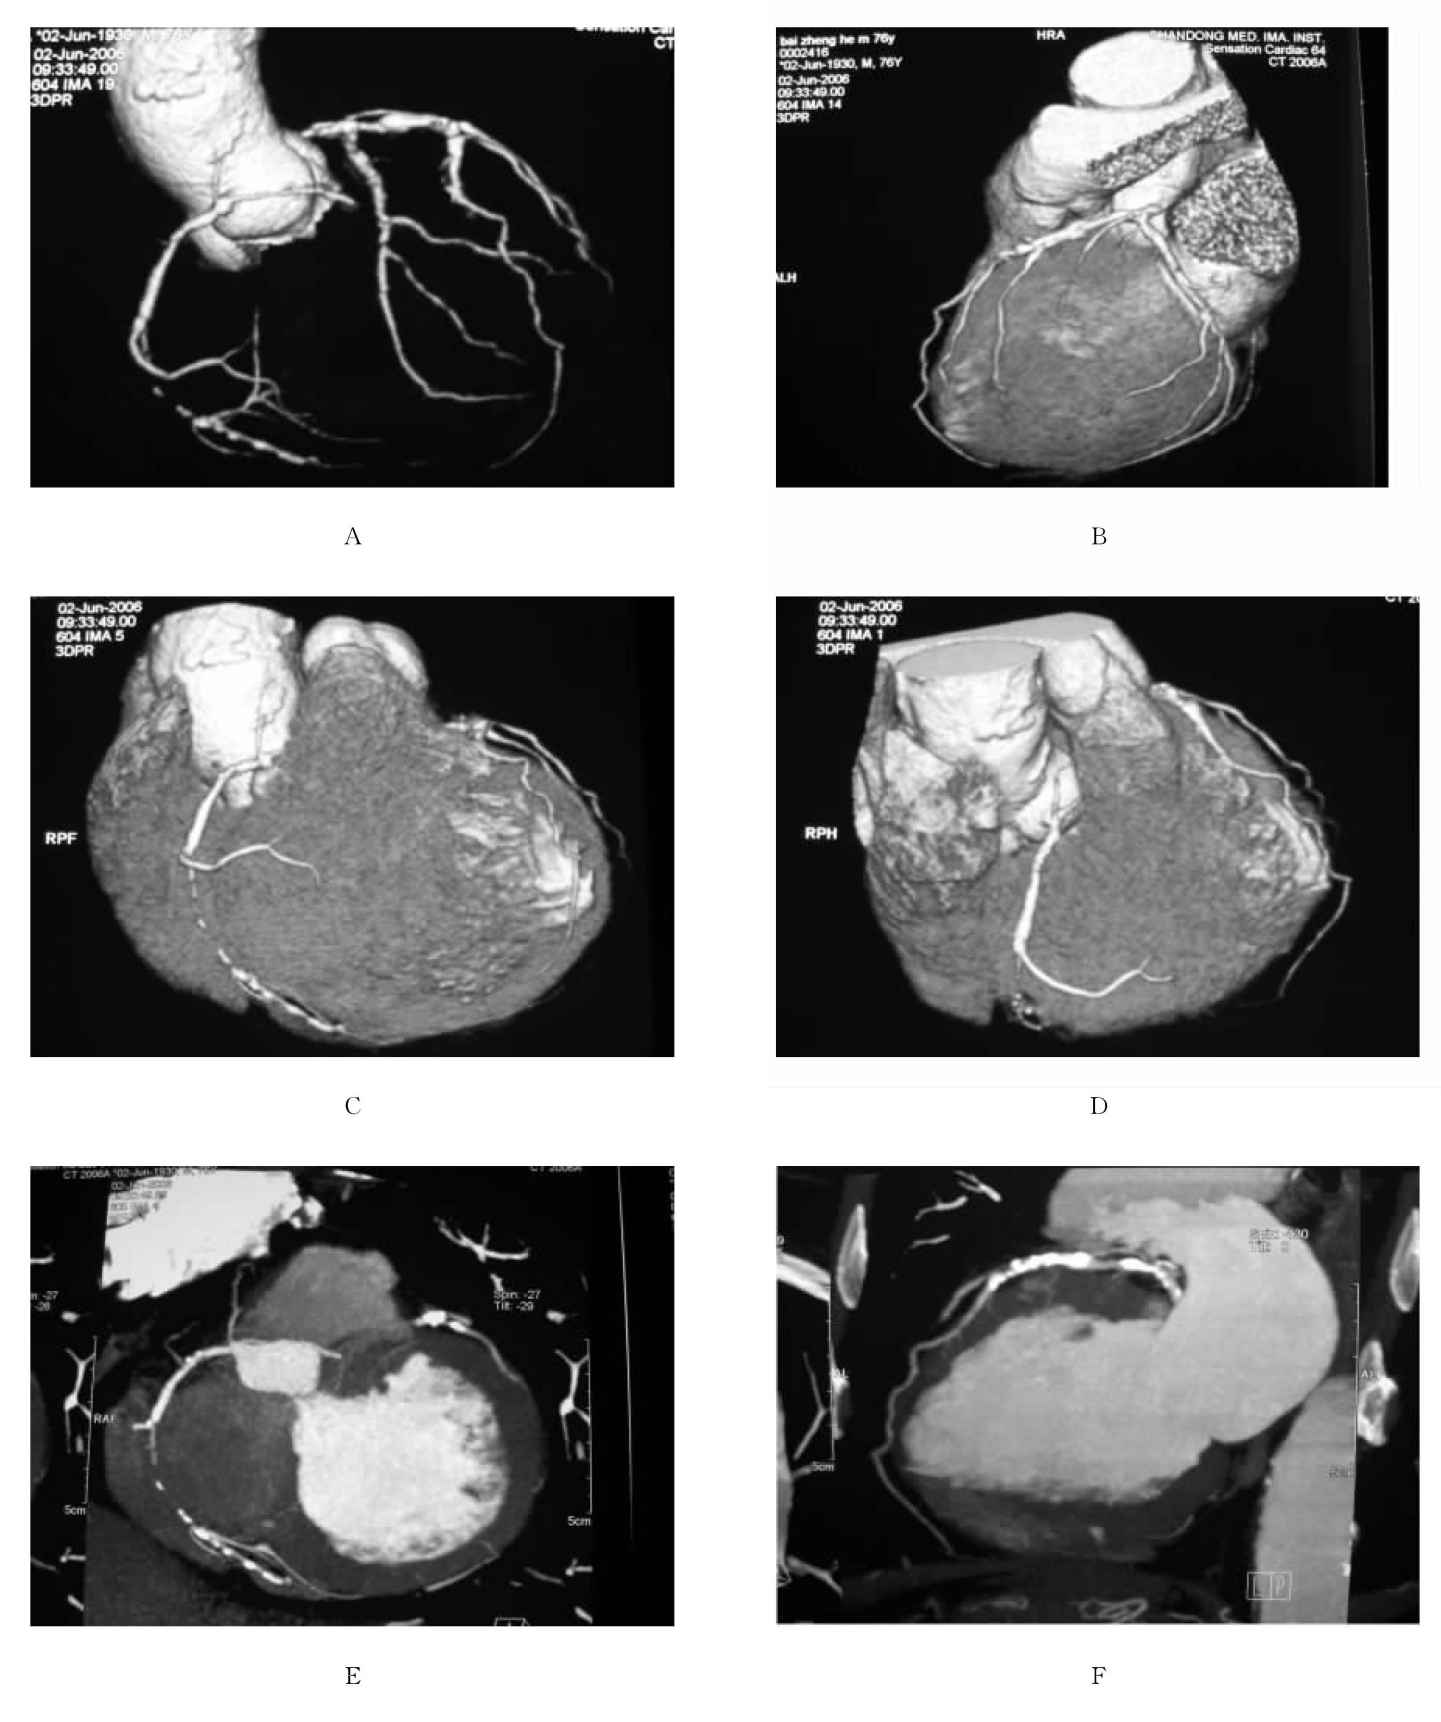
\includegraphics[width=.7\textwidth,height=\textheight,keepaspectratio]{./images/Image00266.jpg}
 \captionsetup{justification=centering}
 \caption{冠状动脉粥样硬化性心脏病\\{\small 左前降支起始处、右冠状动脉有多处狭窄,并可见钙化斑块}}
 \label{fig10-7}
  \end{figure} 

4.心肌梗死及室壁瘤EBCT电影扫描的征象

(1)心肌梗死的主要征象:①局部心肌变薄;②节段性心肌收缩增厚率减低;③室壁运动功能异常:包括运动减弱、消失、矛盾运动或不协调;④整体及局部左室射血分数(EF)减低。

(2)室壁瘤的主要征象:①局部室壁膨凸;②节段室壁薄;③局部矛盾运动;④心腔内附壁血栓所致充盈缺损;⑤整体及局部EF降低。

此外,EBCT和MSCT心肌灌注成像可见梗死区灌注障碍(国外有学者报道正常人心肌灌注量平均为70ml/100g/min,最小值32ml/100g/min,最大值116ml/100g/min),有延迟强化、强化差表现。

5.心肌梗死的主要并发症

①室壁瘤:大范围穿壁性心肌梗死及其后形成的纤维化,受左室内压作用而向外膨出形成室壁瘤,发生率为5%~33%。早期为急性,瘤壁纤维化后形成慢性室壁瘤。80%发生于左室前侧壁,偶位于右室壁,多为单发。室壁瘤可以破裂而致病人死亡。偶有破口小者,破口血肿与心包粘连而形成穿通性室壁瘤即假性室壁瘤。②室间隔穿孔:占心肌梗死的2%~4%。多在急性心肌梗死的早期发生。③乳头肌梗死:心肌梗死几乎均可累及左室乳头肌,出现乳头肌功能不全;严重者腱索断裂,产生严重二尖瓣关闭不全、急性心衰。④心脏破裂。⑤心腔内血栓:常见于左心室内,尤其室壁瘤内。

\subsection{心脏肿瘤}

心脏肿瘤是一种少见疾病,在心脏肿瘤中以转移性多见,是原发性肿瘤的16~40倍。

原发性心脏肿瘤可来自心内膜和心肌。以良性较多,占原发性肿瘤的75%~80%。还有文献将心包肿瘤亦作为心脏肿瘤论述。①来自心膜者:最常见为黏液瘤,还有纤维瘤及各种肉瘤等。②来自心肌者:有脂肪瘤、纤维瘤、平滑肌瘤、畸胎瘤及横纹肌肉瘤等各种肉瘤(见表\ref{tab10-1}),以恶性肉瘤多见。

\begin{table}[htbp]
\centering
\caption{常见的心脏原发肿瘤}
\label{tab10-1}
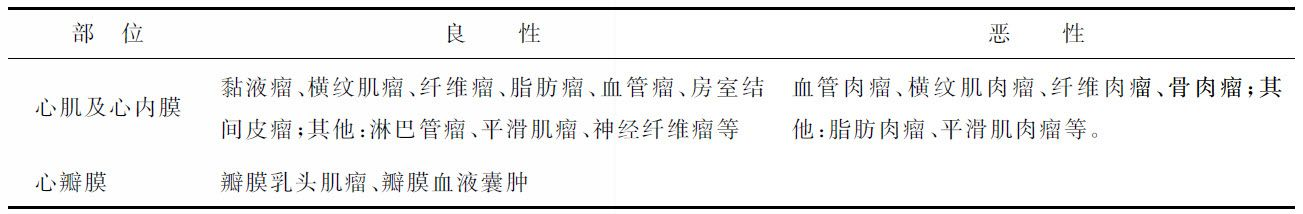
\includegraphics[width=\textwidth,height=\textheight,keepaspectratio]{./images/Image00267.jpg}
\end{table}

最多见的原发良性肿瘤成人为黏液瘤,儿童为横纹肌瘤。最常见的原发恶性肿瘤依次为血管肉瘤、横纹肌肉瘤及间皮瘤。

\subsection{心脏黏液瘤}

本病为最常见的心脏原发性肿瘤,人群发病率为0.5/100万。左心房内占75%,其次为右心房占20%,而左、右心室各占2.5%。

\textbf{【病理】}
大多起源于房间隔卵圆窝附近的原始内皮细胞和心内膜细胞。多为单发,偶可累及多个心腔,一般不会累及心瓣膜。肿瘤常有蒂,呈圆形或分叶状,质软,呈半透明胶冻状,可有出血、钙化。镜下瘤体内含大量黏液样基质,瘤细胞为多边星状细胞,还杂有纤维细胞、平滑肌细胞等。

\textbf{【临床表现】}
好发于30~60岁,女性多于男性。少数为家族遗传性,以青年男性多见,常多发,伴皮肤色素沉着、黑痣等。本病常见的表现为劳累后心慌气短症状,有间歇晕厥史、心衰,心尖部杂音可与体位有关。房室瓣口和(或)心室流出道的梗阻可有猝死的可能,需及时手术。

\textbf{【CT表现】}
因含大量黏液样基质,在瘤性多边星状细胞周边杂以纤维及平滑肌细胞,并伴不同程度的出血、坏死、囊变、纤维变甚至钙化和骨化,故肿瘤密度不均,CT值范围从水样至骨密度。钙化并不少见,有人报道占50%。增强扫描示左心房或右心房内充盈缺损,呈圆形或分叶状,常呈息肉状突起;肿块强化不均,界限不清。总之,位于房间隔或卵圆窝并向心房腔内生长的不均匀肿块,是心房黏液瘤的特征。EBCT电影序列可精确显示瘤体的发生部位、蒂、基底及运动情况。

\textbf{【鉴别诊断】}

1.心内血栓:血栓多附着在左心耳、左心房后侧壁或心尖部;附着面宽,形态不规则,尤其轮廓光滑或呈多个不规则尖角状突起是血栓的特征。其钙化呈层状,增强扫描无强化,动态观察无明显活动。常见有风心病、冠心病或肺心病等心脏疾病。

2.其他肿瘤:黏液瘤密度不均,且低于血液,尤其结合其较特异性的发生部位可予鉴别。如其他肿瘤位于心房近房间隔处则难以鉴别。恶性肿瘤常呈多灶性,心包和心壁易受侵,肺部、纵隔可见转移灶,临床以进行性加重的胸痛和呼吸困难为特征。

\subsection{原发非黏液性良性心脏肿瘤}

\subsubsection{脂肪瘤}

脂肪瘤是最常见的非黏液性心脏良性肿瘤。可发生于任何年龄,以成人多见,男女发病率相近。肿瘤多源于心外膜。瘤体可完全位于心肌内,也可向心腔内外突出。

\textbf{【CT表现】}
位于房间隔或心壁的近脂肪密度肿物、突入心腔或推压心包、无强化为心脏脂肪瘤的重要特点。部分瘤体内可见纤维分隔影。

\subsubsection{纤维瘤}

多发生于儿童及成人,男女发病率相近。左室游离壁前壁、室间隔好发,单发多见。呈卵圆形,由成纤维细胞和胶原纤维构成,质硬、表面光滑、少血供,故密度高、强化轻。可见钙化。

\textbf{【CT表现】}
位于室间隔或其他心壁的单发肿瘤。CT值约60Hu左右、边缘光滑、无明显强化,应首先考虑纤维瘤。肿瘤可见钙化。

\subsubsection{横纹肌瘤}

横纹肌瘤是婴幼儿常见的心脏肿瘤,15岁以上少见。男女之比2∶1。肿瘤常侵犯心室,左右室受累几率相同。90%多发,30%伴结节硬化症。其组织学特征与横纹肌相似,血供丰富。

\textbf{【CT表现】}
肿瘤位于肌壁内,可呈向心腔内突出的多发充盈缺损,边缘光滑或略不规则。增强扫描显著强化,国内报道1例强化值达95Hu,以此可与单发的、强化不著的纤维瘤鉴别。

\subsubsection{淋巴管瘤}

淋巴管瘤由富含淋巴液和淋巴细胞的淋巴管构成,呈海绵状,瘤体含大量淋巴液而不含血管。

\textbf{【CT表现】}
瘤体边缘清楚、呈水样密度或略高于水、无强化,为其重要征象,可有钙化。国内报道1例呈壁内生长,CT值0~15.8Hu。

\subsubsection{血管瘤}

病理分为海绵状血管瘤、毛细血管样血管瘤和动静脉瘘型血管瘤。发病年龄无差异,壁内和腔内生长。

\textbf{【CT表现】}
中、低密度且密度不均的团块影,常见钙化,且明显强化为其特征。有报道可伴有大量心包、胸腔积液。

\subsubsection{起自瓣膜的原发性非黏液性肿瘤}

多见于中年男性。单发、良性、无症状者多,常因瘤块脱落致栓塞、心衰或猝死而被发现。此类肿瘤以乳头弹性纤维瘤最好发,此外,亦可见血管瘤和错构瘤。

\subsection{原发性恶性心脏肿瘤}

\subsubsection{血管肉瘤}

为最常见的原发性心脏恶性肿瘤,常见于右心,60%发生于右房。

\textbf{【临床表现】}
主要表现为心腔及房室瓣口的阻塞症状,可有胸痛、发热、咳嗽等,心包积液有相应症状。

\textbf{【CT表现】}
心腔内条状或分叶状充盈缺损,亦可广泛弥漫浸润性生长,可单发或多发,可向心包侵犯。可并发肺、骨、肝或盆腔等部位转移。

\subsubsection{横纹肌肉瘤}

占第二位,以儿童多见,男女发病率相近。可发生于任何心腔,部分累及心包。

\textbf{【临床表现】}
无特异性,如发热、体重下降等。心脏症状有心律失常、胸痛、瓣膜功能失调、心包积液等。

\textbf{【CT表现】}
肿瘤基部位于心肌,可呈弥漫性浸润心肌或呈息肉样突入心腔内。形态不规则、界限不清,密度不均、可有坏死。肿瘤可多发。受累心肌变形、活动差。累及心包可有心包占位表现和积液。

\subsubsection{淋巴瘤}

50%发生于免疫抑制或获得性免疫缺陷综合征病人,右心房室、心包和纵隔及全身淋巴结受累较多。

\textbf{【临床表现】} 无特异性,如发热、体重下降、胸痛、心包积液等症状。

\textbf{【CT表现】}
心腔内、心包不规则结节及心包、胸腔积液,可伴或不伴纵隔、肺门淋巴结增大。

\subsubsection{纤维肉瘤、脂肪肉瘤或其他肉瘤}

可发生于心脏任何部位,可突入心腔内,常多发。

\textbf{【CT表现】}
生长相对较慢,肿瘤形态不规则,强化多不均匀。亦可侵及心包段胸膜,甚至肺内转移。

\subsection{心脏转移瘤}

心脏转移瘤较原发性多见,除中枢神经系统外,任何器官和组织的恶性肿瘤均可转移至心脏。

\textbf{【病因】}
男性以肺癌,女性以乳癌最多见。肺癌和乳癌多直接侵犯,亦可经淋巴逆行播散至心肌和心包。此外,肾癌和肝癌则常沿下腔静脉进入右房,此亦为肉瘤的主要转移途径。

\textbf{【临床表现】} 主要为心衰、心包积液和心律失常等症状。

\textbf{【CT表现】}
心脏增大、心腔内充盈缺损、心肌壁不规则增厚,同时伴心包转移者见心包积液或(和)心包浸润增厚。如发现胸部或其他部位原发肿瘤有助于诊断。

\section{心包病变}

\subsection{心包积液}

心包积液可分为急性、亚急性和慢性。

\textbf{【病因】}
其病因很多,有感染性、非感染性的,也可为全身疾病的一部分或邻近组织病变蔓延而来。其中常见的是结核性、化脓性、病毒性及非特异性心包炎。此外,还有寄生虫(如原虫)性,以及伴随全身疾病所致的心包炎和心包积液如风湿热、结缔组织疾病、尿毒症、黏液性水肿、脚气病、低蛋白血症、心肌梗塞后综合征、心衰、穿透性损伤、胸导管损伤、出血性疾病、放射损伤、心包肿瘤等。心包积液可分为浆液性、血性、化脓性、浆液纤维蛋白性、乳糜性等。

\textbf{【临床表现】}
心前区疼痛、呼吸困难及其他心包填塞症状,如面色苍白、紫绀、上腹胀痛、浮肿、乏力等。体征为心界扩大、心音遥远,颈静脉怒张,静脉压升高、奇脉(吸停脉)、脉压差降低,肝大、腹水和浮肿等。

\textbf{【CT表现】}

1.少量积液:少量心包积液首先聚集在最低垂部位,常聚集在左心室背侧和左心房的左侧部位,呈一薄层或呈椭圆形液体密度影。

2.中量积液:液体从左心室背侧向上伸展至右心房和右心室的腹侧面(图\ref{fig10-8});积液较多时,可见液体环绕大血管的开口部。

\begin{figure}[!htbp]
 \centering
 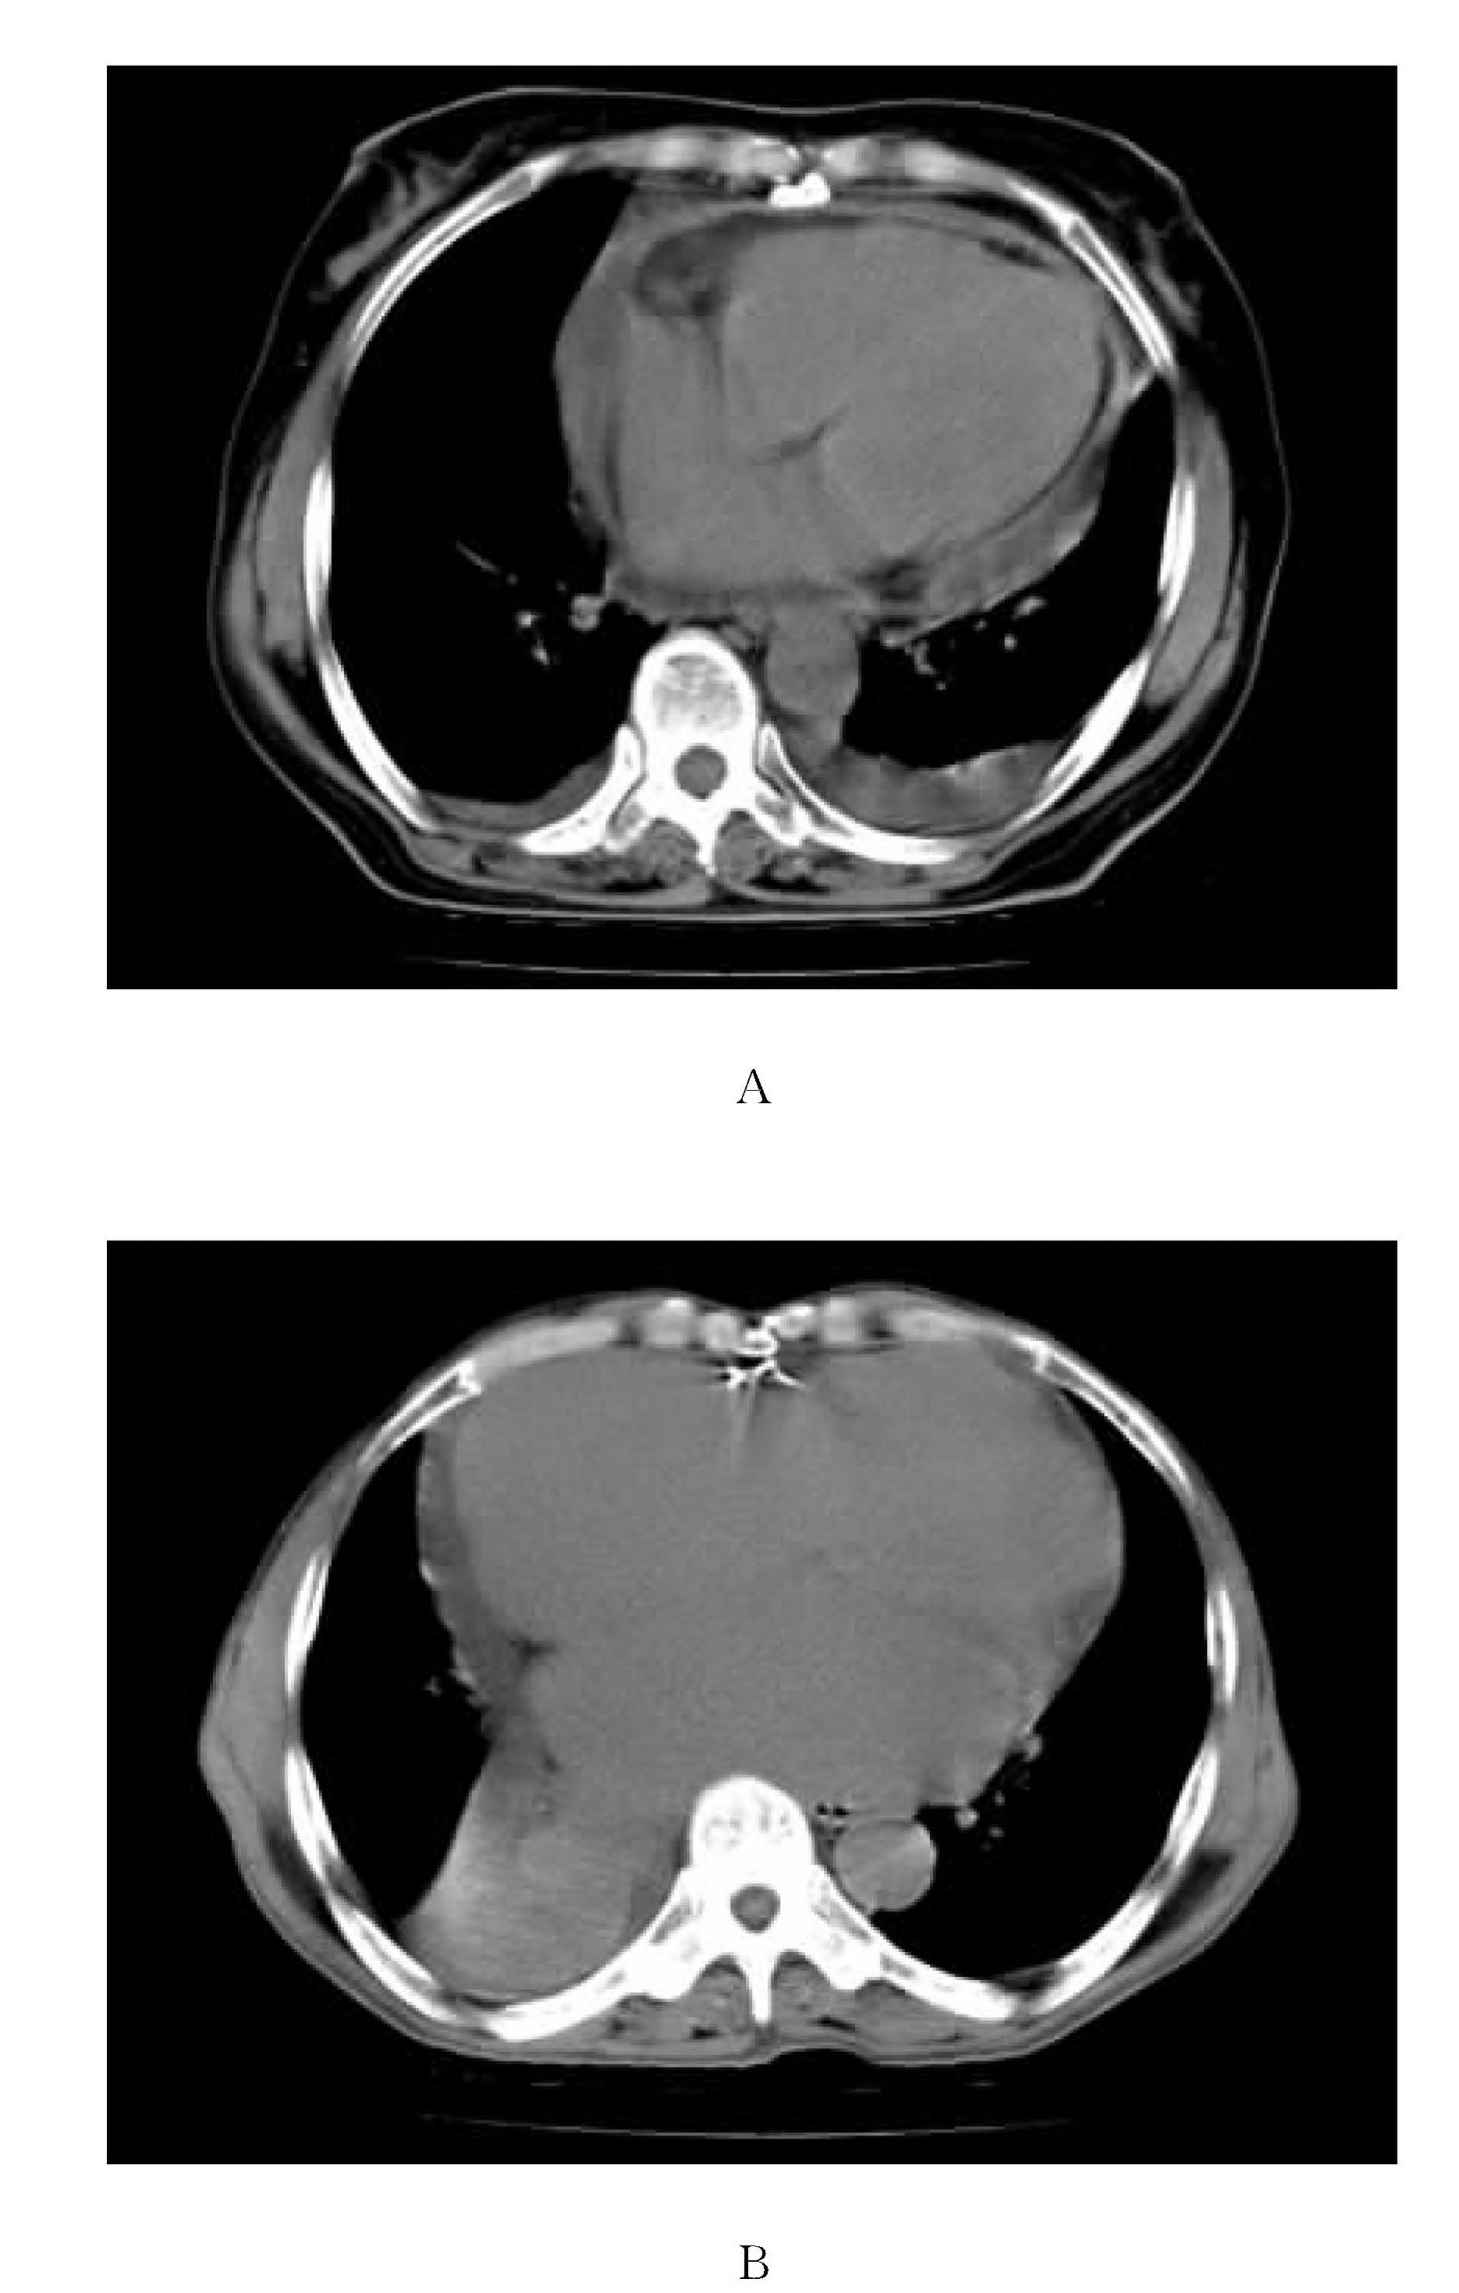
\includegraphics[width=.7\textwidth,height=\textheight,keepaspectratio]{./images/Image00268.jpg}
 \captionsetup{justification=centering}
 \caption{心包积液\\{\small 心脏普大(心衰),心包腔内有中量积液,伴双侧胸水}}
 \label{fig10-8}
  \end{figure} 

3.大量积液:液体充满心包腔,呈不对称的环带状液体密度影环绕心脏和大血管(肺动脉、肺静脉、主动脉及腔静脉)根部。

此外,还有文献报道:取积液最厚处和最薄处值平均,5~15mm为少量,15~25mm为中量,大于25mm为大量。

4.包裹性积液:在心包增厚粘连时,可引起包裹性积液,呈一个或多个局限性液性间隙,常在心脏的背侧和右前方。

5.心包形态改变:主要表现为增厚、粘连。

6.心包积液的密度:①右心功能不全引起的漏出液,具有水样密度,CT值0~20Hu;乳糜液亦可为水样密度;②感染性、肿瘤、慢性肾功能不全等所致者,因含较多蛋白而CT值较高;③心包积血CT值与一般血肿相似,但因心脏搏动的影响,血细胞分离和血红蛋白分解,使其密度不如其他部位的新鲜出血高。

\subsection{缩窄性心包炎}

急性心包炎后,部分患者脏、壁两层粘连增厚,引起心脏舒张功能障碍者,称为缩窄性心包炎。其中,部分病例起病隐匿,并无急性心包炎病史,仅有心包粘连,而心脏功能不受影响者,称为粘连性心包炎。心包积液同时伴有心包增厚、粘连,限制心脏运动,引起功能异常者,称为渗出-缩窄性心包炎。

\textbf{【病因病理】}
缩窄性心包炎的常见病因为结核性、化脓性、病毒性和非特异性炎症,其中以结核性最常见。近年来,心脏手术后的心包缩窄病例越来越多。此外,还可见于创伤性、尿毒症性、心包恶性肿瘤放疗后、风湿热等。缩窄性心包炎病理可见心包有不同程度的不规则增厚、粘连,部分病例可有继发的钙盐沉着形成心包钙化。最有临床意义的两个缩窄部位是心室面的缩窄和房室沟处的缩窄。

\textbf{【临床表现】}
缩窄性心包炎的临床症状可出现在急性心包炎后数月至数年。主要表现为心悸、气急、乏力和腹胀等。体检可见颈静脉怒张,静脉压升高、肝大、腹水和下肢浮肿等。

\textbf{【CT表现】}
对于心包增厚及钙化平扫即可;增强扫描可用于观察室间隔扭曲成角、心室腔畸形以及鉴别心包增厚与少量积液等。①心包增厚:最具诊断意义,可数毫米至数厘米不等。心包厚度>3mm(或4mm)有意义,部分可伴局限性单个或多个包裹性积液。②心包钙化:呈斑点状、结节状、斑片状、线状或大片状。脏层钙化多分布于房室沟、室间沟和交叉沟处;壁层钙化多见于右室腹侧面及心膈面,但不易区分脏、壁两层。③下腔静脉扩张:正常<3cm,心包增厚与下腔静脉扩张同时存在时,表明心包病变损害了心脏的舒张充盈,提示缩窄性心包炎存在。④室间隔扭曲或远端呈锐角:具有特异性。⑤心室轮廓受压变形。⑥心房扩大:可为左房或(和)右房扩大。⑦胸腔积液:伴单侧或双侧胸腔积液者可占50%~71%,一般认为是继发的血液动力学改变的结果。⑧右心房血栓形成:少见。

总之,心包增厚、室间隔扭曲成角及下腔静脉扩张等征象最为重要。3种征象同时出现或心包增厚伴后两者之一,可诊断为缩窄性心包炎。

\textbf{【鉴别诊断】}

1.粘连性心包炎:可有心包增厚,甚至心包钙化。但这种病例的下腔静脉影无明显扩张等,临床上无缩窄性心包炎的血液动力学变化。

2.限制型心肌病:临床上与缩窄性心包炎不易鉴别。而后者可清楚显示心包的增厚及钙化是鉴别的关键,但心包厚度在2~3mm者,常需活检证实。

3.少量心包积液:一般平扫时心包增厚的CT值高于积液;如有钙化或心包呈不规则结节状改变,则支持心包增厚。必要时增强扫描,CT值升高较明显者应为心包增厚。

\subsection{心包间皮瘤}

心包原发性肿瘤比心脏的原发性肿瘤少见,而心包转移性肿瘤要比心肌受侵犯常见。原发性心包肿瘤明显比转移性少见。原发性心包肿瘤中半数为恶性,其中以间皮瘤常见。心包良性肿瘤有心包囊肿、脂肪瘤、畸胎瘤、支气管囊肿、平滑肌瘤和血管瘤等(见表\ref{tab10-2})。

\begin{table}[htbp]
\centering
\caption{常见的心包原发肿瘤}
\label{tab10-2}
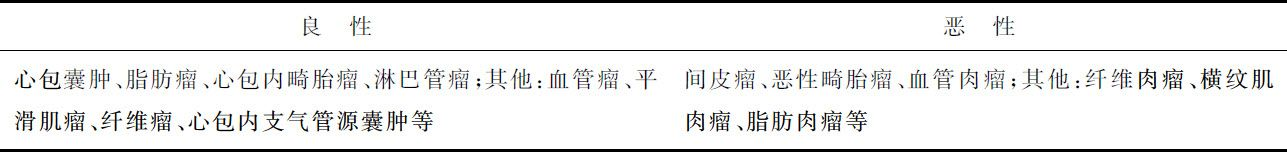
\includegraphics[width=\textwidth,height=\textheight,keepaspectratio]{./images/Image00269.jpg}
\end{table}

\textbf{【病理】}
间皮瘤可为单个或多个斑块状实质性肿块,发生于脏层和壁层心包,可伴心包积液、积血和心包缩窄。本病除原发外,很多由胸膜间皮瘤转移而来,但有时确定原发部位较难。

\textbf{【临床表现】}
缺乏特异性。心力衰竭、心律失常、心脏填塞和缩窄性心包炎的症状。

\textbf{【CT表现】}
心间皮瘤表现为心包腔内单个或多个软组织结节,或为不规则心包增厚,可伴有或不伴心包积液。常侵犯胸膜、腹膜,心肌内浸润和播散少。如同时存在石棉肺、胸膜间皮瘤,可出现相应表现。

\subsection{心包转移瘤}

恶性肿瘤侵犯或转移到心脏和心包有3条途径,即从邻近器官的直接侵犯、血行转移和淋巴转移。肺癌、乳癌是累及心脏和心包的主要肿瘤,其次为淋巴瘤、黑色素瘤等。

\textbf{【临床表现】}
也缺乏特异性。可有心律失常、心包填塞等症状,可有原发癌的病史和症状。

\textbf{【CT表现】}
无特异性。主要表现为心包积液、积血,积液的CT值偏高。也可伴心包局限性或普遍性增厚,以及多个结节或肿块附着于心包上。

\textbf{【鉴别诊断】}
心包转移性和原发性恶性肿瘤的CT表现相似,鉴别诊断需密切结合病史。

\section{心脏及胸部大血管损伤}

\subsection{心脏外伤}

心脏外伤可分为钝挫伤和穿透性损伤两类。在钝挫伤中较常见的为心包损伤引起的出血或心包积液,多合并肋骨骨折、血气胸或肺挫伤。

\textbf{【病理机制】}
①胸骨与胸椎压迫心脏使之破裂;②直接或间接的胸内压突然增加而致心脏破裂;③心脏挫伤、心肌软化坏死致心脏迟发性破裂;也有人认为心脏迟发性破裂是心内膜撕裂的结果;④心肌梗死:冠状动脉损伤所致;⑤枪击伤或刺伤直接损伤心脏。

\textbf{【临床表现】}
严重挫伤导致的心肌挫伤及心脏破裂大多当即死亡。患者常感胸痛及呼吸困难外,听诊心音遥远、心搏动微弱,低血压,颈静脉怒张等。

\textbf{【CT表现】}
严重挫伤所致的心脏破裂,平扫可见高密度心包积血及胸腔积血。穿透性损伤中,被锐器刺伤的心脏可自行封闭导致心包填塞而无大量出血;如仅刺伤心包,可引起心包积气和(或)出血,而CT表现为心包积气或液气心包。

\subsection{胸主动脉及大血管损伤}

\textbf{【病因病机】}
其病因多见于交通事故突然减速、胸部受方向盘的撞击或被抛出车外的人,以及高空坠落者。损伤机理包括血管的剪切力和断骨片的直接作用。主动脉峡部是剪切伤所致撕裂的最好发部位,约占85%。当发生第一肋骨、锁骨骨折时,可损伤锁骨下动脉、无名动脉及颈总动脉。

\textbf{【临床表现】}
因常伴有胸部多发性以及胸腹部和盆腔多器官损伤,临床表现多样化。可有胸骨后疼痛、背痛、呼吸困难等。约1/3伤者有上肢高血压、下肢低血压,较具特征性。

\textbf{【CT表现】}
平扫可见等密度或稍高密度的圆形、椭圆形影,但难以区分是假性动脉瘤或纵隔血肿。增强扫描可表现为以下一个或多个征象。①假性动脉瘤:位于主动脉弓旁、破口小者瘤体强化明显迟于主动脉并排空延迟即“晚进晚出征”;破口大者这种时间差不著;②主动脉夹层分离;③血管边缘不规则,壁厚薄不均;④主动脉周围血肿:常见,无强化,紧贴主动脉者高度提示主动脉撕裂;远离者多为小血管破裂;⑤其他:如气管、食管推挤移位,胸骨、胸椎及第1~3肋骨骨折等,均提示有胸主动脉及大的分支损伤可能。

目前,各种影像难以鉴别主动脉内膜轻微损伤与主动脉粥样硬化。

\protect\hypertarget{text00018.html}{}{}

